% %%%%%%%%%%%%%%%%%%%%%%%%%%%%%%%%%%%%%%%%%%%%%%%%%%%%%%%%%%%%%%%%%%%%%%%%%%%%%
% thesis.tex: Primary TeX control file for thesis.
% %%%%%%%%%%%%%%%%%%%%%%%%%%%%%%%%%%%%%%%%%%%%%%%%%%%%%%%%%%%%%%%%%%%%%%%%%%%%%
\documentclass[11pt, oneside]{mnthesis}
\usepackage{epsfig} % Allows the inclusion of eps files
\usepackage{epic} % Enhanced picture mode
\usepackage{eepic} % Extensions for epic
\usepackage{units} % SI unit typesetting
\usepackage{url} % URL handling
\usepackage{longtable} % Tables that continue onto multiple pages
\usepackage{mathrsfs} % Support for \mathscr script
\usepackage{multirow} % Span rows in tables
%\usepackage{bigstrut} % Space struts in tables up and down
\usepackage{amssymb} % AMS math symbols and helpers
\usepackage{graphicx} % Enhanced graphics support
\usepackage{setspace} % Adjust spacing in captions, single by default
\usepackage{xspace} % Automatically adjusting space after macros
\usepackage{amsmath} % \text, and other math formatting options
\usepackage{siunitx} % \num{} formatting and SI unit formatting
\usepackage{booktabs} % Enhanced tables with \toprule, etc.
\usepackage{hyperref} % Add clickable links to other parts of the document
\usepackage[noabbrev,capitalize]{cleveref} % Automatically determine \cref type

\usepackage[hang,flushmargin]{footmisc} % Prevent indent in footnotes. 

% Put captions tighter to their figures. Not clear if it actually works. 
\setlength{\abovecaptionskip}{0pt}

\usepackage{xcolor} % so we can put todo notes in color. 

\usepackage{doi} % Link to doi in the bibliography. Doesn't seem to work. 

\usepackage{parskip} % http://ctan.org/pkg/parskip vskip instead of indent. 

\usepackage{float} % Sometimes you want to tell LaTeX to put an image RIGHT HERE. 

% Prevent LaTeX from putting a figure right before the start of a section. 
\usepackage[section]{placeins}


% Configure the siunitx package
\sisetup{
    group-separator = {,}, % Use , to separate groups of digits, like 12,345
    list-final-separator = {, and } % Always use the serial comma in \SIlist
}

% Configure the cleveref package
\newcommand{\creflastconjunction}{, and } % Always use the serial comma




\newcommand{\Alfven}{Alfv\'en\xspace}

\newcommand{\Ampere}{Amp\`ere\xspace}

\newcommand{\xhat}{\ensuremath{\hat{x}}\xspace}
\newcommand{\yhat}{\ensuremath{\hat{y}}\xspace}
\newcommand{\zhat}{\ensuremath{\hat{z}}\xspace}

\DeclareSIUnit\RE{R_E}

\renewcommand{\vec}[1]{\underline{#1}}

\newcommand{\tensor}[1]{\underline{\underline{#1}}}

\newcommand{\dd}[1]{\ensuremath{ \frac{\partial}{\partial #1} }\xspace}

\newcommand{\ddt}{\dd{t}\xspace}

\newcommand{\dt}{\ensuremath{\delta \hspace{-0.1em} t} \xspace}

\newcommand{\curl}[1]{\ensuremath{ \nabla \times \vec{#1} }\xspace}

\newcommand{\lr}[1]{ \left( #1 \right) }

\newcommand{\lrsmall}[1]{ \left( {\scriptstyle #1} \right) }

\renewcommand{\arg}[1]{\!\lr{#1}}

\newcommand{\argsmall}[1]{\!\lrsmall{#1}}



\newcommand{\mmm}[9]{ \left[ \begin{array}{ccc}
    #1 & #2 & #3 \\
    #4 & #5 & #6 \\
    #7 & #8 & #9
  \end{array} \right] }

\newcommand{\mm}[4]{ \left[ \begin{array}{cc}
    #1 & #2 \\
    #3 & #4
  \end{array} \right] }

\newcommand{\vv}[2]{ \left[ \begin{array}{c}
    #1 \\
    #2
  \end{array} \right] }






% Note: Do we want to squish dt together? Do we want to always have tiny spaces
% between variables being multiplied together? 
\newcommand{\deltat}{\delta \hspace{-0.1em} t}


% Physics constants
\newcommand{\C}{{\mathrm{c}}}

% Add space between rows of tables
\newcommand{\spacerows}[1]{\renewcommand{\arraystretch}{#1}}

% Define a better looking eV by moving the V slightly left
\DeclareSIUnit\electronvolt{e\hspace{-0.08em}V}


\linespread{1.3}

% Compile only the chapters listed here. This may make the compile faster, but
% it's not necessary. 
%\includeonly{
%    preliminaries/title,
%    chapters/intro,
%    chapters/model,
%    chapters/math,
%    chapters/results,
%    chapters/data,
%    chapters/conclusion,
%    chapters/app_geometry,
%    chapters/app_integrating,
%}



% %%%%%%%%%%%%%%%%%%%%%%%%%%%%%%%%%%%%%%%%%%%%%%%%%%%%%%%%%%%%%%%%%%%%%%%%%%%%%
% %%%%%%%%%%%%%%%%%%%%%%%%%%%%%%%%%%%%%%%%%%%%%%%%%%%%%%% Mark this as a draft. 
% %%%%%%%%%%%%%%%%%%%%%%%%%%%%%%%%%%%%%%%%%%%%%%%%%%%%%%%%%%%%%%%%%%%%%%%%%%%%%
\draft
% %%%%%%%%%%%%%%%%%%%%%%%%%%%%%%%%%%%%%%%%%%%%%%%%%%%%%%%%%%%%%%%%%%%%%%%%%%%%%
% %%%%%%%%%%%%%%%%%%%%%%%%%%%%%%%%%%%%%%%%%%%%%%%%%%%%%%%%%%%%%%%%%%%%%%%%%%%%%
% %%%%%%%%%%%%%%%%%%%%%%%%%%%%%%%%%%%%%%%%%%%%%%%%%%%%%%%%%%%%%%%%%%%%%%%%%%%%%



\begin{document}
%\bibliographystyle{hunsrt} % Default bibliography style file moved to archive/
\bibliographystyle{abbrv}

% Title and other sections that come before the body of the document
\include{preliminaries/title}


% Introductory chapters. 
% %%%%%%%%%%%%%%%%%%%%%%%%%%%%%%%%%%%%%%%%%%%%%%%%%%%%%%%%%%%%%%%%%%%%%%%%%%%%%
% %%%%%%%%%%%%%%%%%%%%%%%%%%%%%%%%%%%%%%%% Survey of the Near-Earth Environment
% %%%%%%%%%%%%%%%%%%%%%%%%%%%%%%%%%%%%%%%%%%%%%%%%%%%%%%%%%%%%%%%%%%%%%%%%%%%%%

\chapter{The Near-Earth Environment}
\label{ch_intro}

It's all about energy transfer! 

Some example citations, including a few with special characters: \cite{dai_2013}, \cite{dai_2015}, \cite{lysak_2001}. 

%There are a lot of interrelated things going on, so it's hard to describe Earth's environment one step at a time. Look at Scott's thesis -- he did this well, right? 

%Heliosphere, Magnetosphere, Ionosphere, Atmosphere?

%Current systems, convective systems, density profiles? 

%\begin{figure}
%  \includegraphics[width=5.75in, height=2in]{figures/image.jpg}
%  \caption{Lorem ipsum dolor sit amet, consectetur adipiscing elit, sed do eiusmod tempor incididunt ut labore et dolore magna aliqua.}
%  \label{fig_test}
%\end{figure}

Sun generates energy through nuclear reactions. 

This energy drives behavior in the near-Earth environment. 

Typical solar wind density is $\sim$ \SI{5}{/\cm\cubed}. Typical solar wind velocity at Earth is \SIrange{e2}{e3}{\km/\s}. Typical solar wind particle energy is \SIrange{1}{10}{\kilo\eV}. Density can vary by $\sim$3 orders of magnitude, and velocity by one, during times of high solar activity. CMEs can also mess with the north/south component of the interplanetary magnetic field. 

\SI{45}{\degree} angle with the Earth-Sun line, which is the \X direction. 
\footnote{We use uppercase \X, \Y, and \Z to indicate GSE coordinates: \X points from the Earth to the Sun. \Y is perpendicular to \X, and in the Sun's ecliptic plane, pointing duskwards... against Earth's orbital motion. Points north, out of the ecliptic plane. Later, we will use lowercase \x, \y, and \z to define a more-or-less analogous corodinate system with respect to Earth.}

Solar wind is what deforms Earth's magnetic field to form the magnetosphere. 

Transient solar wind phenomena, such as coronal mass ejections, are also known to be related to geomagnetic disturbances at Earth. Jesse cites here: 

R. L. McPherron. Physical processes producing magnetospheric substorms and mangetic storms. In J. A. Jacobs, editor, Geomagnetism, volume 4, chapter 7. Academic Press, 1991.

G. Rostoker. Substorms. In Handbook of the Solar-Terrestrial Environment, chapter 15. Springer-Verlag, 2007.

This might just be worth tracking down... Jesse cites several chapters: 

M. Shulz. Magnetospheres. In Handbook of the Solar-Terrestrial Environment, chapter 7. Springer-Verlag, 2007.


% papers mentioned during Yan's talk. mostly about alfven acceleration and nonlinear effects. 
% Vasyliunas 1970, 1984
% Hasegawa 1976
% Goertz 1991
% Stasiewicz et al 2000
% Haerendel 2008
% Song & Lysak 1994, 1999, 2000, 2001, 2006, 2011, 2012
% Inverted V?
% Double layers? 
% Charge holes? 



% =============================================================================
% =============================================================================
% =============================================================================
\section{The Outer Magnetosphere}

The outer magnetosphere is a region where the field lines are closed, but significantly deformed by the solar wind. 

\subsection{The Magnetopause}

\subsection{The Magnetotail}

\subsection{Cusp Regions}

% =============================================================================
% =============================================================================
% =============================================================================
\section{The Inner Magnetosphere}

In the inner magnetosphere, field lines are closed, and are approximately dipolar. 

\subsection{The Plasmasphere}

\subsection{Ring Currents}

\subsection{The Radiation Belts}

% =============================================================================
% =============================================================================
% =============================================================================
\section{The Ionosphere}

The ionosphere is immediately above Earth's neutral atmosphere. 

\subsection{Field-Aligned Currents}

\subsection{Pedersen and Hall Currents}

\subsection{Particle Precipitation}

% =============================================================================
% =============================================================================
% =============================================================================
\section{Geomagnetic Disturbances}

\subsection{Storms}

\subsection{Substorms}










\chapter{The Near-Earth Environment}
  \label{ch_environment}

%ALEX NOTES
%## Chapter 2
%### 2.1
%- I'm not sure what "width" and "length" means when measuring a magnetosphere.
%- I wonder if I have any relation to this Dungey... That's my mother's maiden
%  name.
%### 2.2
%- I think standard practice is to use em dashes without spaces.

From Earth's surface to a height of a hundred kilometers or so, the atmosphere
is a well-behaved fluid: a collisional ensemble of neutral atoms. Higher up,
its behavior changes dramatically. As altitude increases, solar ultraviolet
radiation becomes more intense, which ionizes atmospheric atoms and molecules.
Density also decreases, slowing collisional recombination. Whereas the neutral
atmosphere is held against Earth's surface by gravity, the motion of charged
particles is dominated by Earth's geomagnetic field, as well as the
electromagnetic disturbances created as that field is hammered by the solar
wind. 

Before discussing specific interactions, it's appropriate to introduce the
so-called ``frozen-in condition.'' In a collisionless plasma, magnetic field
lines are equiputential contours. Charged particles move freely along the
contours, but cannot move across them. Compression of the magnetic field is
synonymous with compression of the ambient plasma, as any magnetic field lines
that thread a moving plasma are dragged along with it. This assumption is valid
throughout most of the magnetosphere --- that is, the region of space primarily
governed by Earth's magnetic field --- and provides an invaluable tool for
understanding the large-scale motions of plasmas and fields. 

%\todo{Neutral density is larger than charged particle density (?) but it doesn't matter because mean free path is huge. }

% -----------------------------------------------------------------------------
% -----------------------------------------------------------------------------
% -----------------------------------------------------------------------------
\section{The Outer Magnetosphere}
  \label{sec_outer}

%\footnote{In the case of an ideal plasma, \ohmlaw takes the form $\vec{E} + \vec{U} \times \vec{B} = 0$. }. 

%\todo{Jets from magnetic reconnection... release of magnetic tension! }

Plasma behavior within Earth's magnetosphere is ultimately driven by the solar
wind: a hot (\about\SI{100}{\eV}), fast-moving (\about\SI{100}{\km/\s}) plasma
threaded by the interplanetary magnetic field
(\about\SI{10}{\nT})\footnote{Listed values correspond to the solar wind at
Earth's orbit. }. The density of the solar wind is on the order of
\SI{10}{\percc}; in a laboratory setting, this would constitute an ultra-high
vacuum (atmospheric density at sea level is \about\SI{e19}{\percc}), but
compared to much of the magnetopause it's quite dense. 

\begin{figure}[!htb]
  \centering
  \includegraphics[width=\textwidth]{figures/outer_magnetosphere.pdf}
  \caption[Reconnection in the Outer Magnetosphere]{
    When the solar wind magnetic field (red) points southward, reconnection can
    occur between it and Earth's (northward) closed magnetic field lines
    (blue). The resulting open field lines (magenta) convect nightward over the
    poles, ultimately arriving in the magnetotail. There, the open field lines
    reconnect again. Newly closed field lines move Earthward, carrying flux
    across the flanks and back to the dayside. The rest are completely
    decoupled from Earth, and are lost to the solar wind. 
  }
  \label{fig_outer_magnetosphere}
\end{figure}

The magnetosphere's outer boundary represents a balance between the solar wind
dynamic pressure and the magnetic pressure of Earth's dipole field. On the
dayside, the dipole is compressed, pushing this boundary to within about
\SI{10}{\RE} of Earth\footnote{Distances in the magnetosphere are typically
measured in units of Earth radii: $\SI{1}{\RE} \equiv \SI{6378}{\km}$. }. The
nightside magnetosphere is stretched into a long tail which may exceed
\SI{50}{\RE} in width and \SI{100}{\RE} in length. 

When the interplanetary magnetic field opposes the geomagnetic field at the
nose of the magnetosphere, magnetic reconnection occurs. Closed magnetospheric
field lines ``break,'' opening up to the interplanetary magnetic
field\footnote{Closed field lines are more or less dipolar; one end connects to
the north pole of Earth's magnetic core, and the other end to the south pole.
Open field lines are tethered to Earth at one end. In principle, the other end
eventually doubles back to Earth, but for practical purposes it is lost to the
solar wind. The distinction is important because charged particle motion is
guided by magnetic field lines, as discussed in \cref{ch_flrs}. }. They then
move tailward across the poles, dragging their frozen-in plasma with them.
Reconnection in the tail allows magnetic field lines to convect back to the day
side, across the flanks. This process is called the Dungey
cycle\cite{dungey_1961}. 

Viewed from the north, the Dungey cycle involves a clockwise flow of flux and
plasma on the dusk side and a counterclockwise flow on the dusk side. The
motion is accompanied by a convection electric field, per \ohmlaw in an ideal
plasma:
\begin{align}
  \vec{E} + \vec{U} \times \vec{B} = 0
\end{align}

Where \vec{B}, \vec{E}, and \vec{U} are the magnetic field, electric field, and
plasma velocity vectors respectively. 

Consistent with \amplaw, the interplanetary magnetic field is separated from
the magnetosphere by a current sheet: the magnetopause. On the dayside, the
magnetopause current flows duskward; on the nightside, it flows dawnward around
the magnetotail. 

Earth's dipole is significantly deformed in the magnetotail; field lines in the
northern lobe of the tail points more or less Earthward, and vice versa. Plasma
within the lobes is cool (\about\SI{100}{\eV}) and rarefied
(\about\SI{e-2}{\percc}). The two lobes are divided by the plasma sheet, which
is comparably hot (\about\SI{e3}{\eV}) and dense (\about\SI{1}{\percc}). The
plasma sheet carries a duskward current which connects to the magnetopause
current. 

% -----------------------------------------------------------------------------
% -----------------------------------------------------------------------------
% -----------------------------------------------------------------------------
\section{The Inner Magnetosphere}

Within $L \sim 8$ (where $L$ is the McIlwain parameter\footnote{The McIlwain
parameter $L$ is used to index field lines in Earth's dipole geometry:
$L \equiv \frac{r}{\sin^2\theta}$ for colatitude $\theta$ and radius $r$ in
Earth radii. For example, the $L=5$ field line passes through the equatorial
plane at a geocentric radius of \SI{5}{\RE}, then meets the Earth at a
colatitude of $\arcsin \sqrt{ \frac{1}{5} } \sim \SI{27}{\degree}$ (equally, a
latitude of $\arccos \sqrt{ \frac{1}{5} } \sim \SI{63}{\degree}$). }), the
dipole magnetic field is not appreciably deformed by the solar wind. As a
result, the structures in the inner magnetosphere follow closely from the
motion of charged particles in an ideal dipole field. 

\begin{figure}[!htb]
  \centering
  \includegraphics[width=\textwidth]{figures/inner_magnetosphere.pdf}
  \caption[Structures in the Inner Magnetosphere]{
    The above figure shows typical ranges in $L$ for the plasmasphere (red,
    $L < 4$), ring current (green, $3 < L < 5$) and radiation belts (blue,
    $L < 2$ and $4 < L < 6$). These values, particularly the size of the
    plasmasphere, can vary significantly in response to geomagnetic activity. 
  }
  \label{fig_inner_magnetosphere}
\end{figure}

The plasmasphere --- a cold (\about\SI{1}{\eV}), dense
(\SIrange{e2}{e4}{\percc}) torus of corotating plasma --- is formed by the
outward drift of atmospheric ions along magnetic closed field lines. Its outer
boundary is thought to represent a balance between the corotation electric
field (per the rotation of Earth's magnetic dipole) and the convection electric
field (associated with the convection of magnetic flux during the Dungey
cycle). Particle density drops sharply at the edge of the plasmasphere; the
boundary is called the plasmapause. The plasmapause typically falls around
$L=4$, though during prolonged quiet times it can extend to $L=6$ or larger. 

Energetic particles trapped within the inner magnetosphere are divided into two
populations. 

The Van Allen radiation belts are made up of particles with energy above
\SI{e5}{\eV} or so. The inner belt ($L\lesssim2$) is primarily composed of
protons, the decay remnants of neutrons freed from the atmosphere by cosmic
rays. The outer belt ($L\gtrsim4$) is primarily composed of high-energy
electrons. The density of radiation belt particles is significantly affected by
geomagnetic storms and substorms; a typical value is \SI{10}{\percc}. 

Particles with energies of \SIrange{e3}{e5}{\eV} make up the ring current,
which extends from $L\sim3$ to $L\sim5$. Gradient-curvature drift carries ions
and electrons in opposite directions; the net result is a westward current.
During quiet times, the ring current causes magnetic a southward magnetic field
on the order of \SI{1}{\nT} at Earth's equator, while during geomagnetically
active times (discussed in \cref{sec_storms}) the effect may be \SI{100}{\nT}
or more\footnote{For comparison, Earth's dipole field points north at the
equator with a magnitude over \SI{e4}{\nT}. }. 

% -----------------------------------------------------------------------------
% -----------------------------------------------------------------------------
% -----------------------------------------------------------------------------
\section{The Ionosphere}
  \label{sec_ionos}

Earth's neutral atmosphere is an excellent insulator. Collisions are so
frequent that charged particles quickly thermalize and recombine. The breakdown
of air molecules into a conductive plasma (as happens during a lightning
strike, for example) requires electric fields on the order of \SI{e9}{\mV/\m}. 

Cold particles in the magnetosphere are likewise not conducive to currents. In
the absence of collisions, electrons and ions drift alongside one another in
response to an electric field, creating no net current perpendicular to the
magnetic field\footnote{The so-called $E$-cross-$B$ drift is associated with a
velocity of $\vec{U} = \frac{1}{B^2} \vec{E} \times \vec{B}$, independent of a
charged particle's mass or sign. }. Magnetic field lines can typically be
considered as equipotential contours, devoid of field-aligned potential
structures. 

The ionosphere is a sweet spot between the two regimes. Collisions are frequent
enough to disrupt the drift of ions, but not frequent enough to immobilize the
electrons. The result is a finite-valued conductivity tensor. Pedersen currents
(which scale with the Pedersen conductivity) flow in the direction of the
perpendicular electric field. Hall currents (due to the Hall conductivity) flow
in the $\vec{B} \times \vec{E}$. It is these currents --- particularly the Hall
current --- which give rise to magnetic fields at the ground. Collisions in the
ionosphere also result in a finite parallel conductivity, allowing for the
formation of potential structures along the magnetic field line. 

%\todo{Field-aligned currents depend on the level of geomagnetic activity... but do they ever completely go away? }

The convection electric field (associated with the Dungey cycle,
\cref{sec_outer}) drives Pedersen currents in the ionosphere. Pedersen currents
flow dawnward on the flanks and duskward across the poles. The currents remain
divergence-free by connecting to field-aligned currents at the edges of the
polar cap. The field-aligned currents, in turn, connect to the magnetopause
current, the cross-tail current, and the (partial) ring current. 

When electron density is low, thermal velocities may be unable to carry enough
current to satisfy $\nabla \cdot \vec{J} = 0$. This leads to the formation of
potential structures along geomagnetic field lines in the ionosphere. Such
structures accelerate particles along magnetic field lines, leading to the
precipitation of energetic particles into the atmosphere. As the particles
thermalize, they excite atmospheric atoms. The resulting spontaneous emission
is often in the visible spectrum, giving rise to the aurora. 

%\todo{Particles can also be excited by \Alfven waves... this probably goes in \cref{ch_flrs}. }

%From \cite{paschmann_2003}: ``In the thermosphere, the solar ultraviolet (UV) light and energetic particles precipitating from the magnetosphere produce ionization increasing with altitude. At the same time the particle density is low enough to make the recombination times of the ionized atoms and molecules sufficiently long to allow a significant fraction of the gas to remain ionized. This produces a conducting layer of the atmosphere known as the ionosphere. The ionosphere begins at $\sim\SI{65}{\km}$, has a peak plasma density between 200 and 300 km, and eventually merges with magnetospheric regions $\sim$1000--2000 km altitudes.''

%The effects of mean molecular mass on conductivity are computed per the usual definitions. 
%\begin{align}
%  \sp &= \displaystyle\sum_s \frac{n_s q_s^2}{m_s} \frac{\nu_s}{\nu_s^2 + \Omega_s^2} &
%  \sh &= -\displaystyle\sum_s \frac{n_s q_s^2}{m_s} \frac{\Omega_s}{\nu_s^2 + \Omega_s^2} &
%  \sz &= \displaystyle\sum_s \frac{n_s q_s^2}{m_s \nu_s}
%\end{align}

% -----------------------------------------------------------------------------
% -----------------------------------------------------------------------------
% -----------------------------------------------------------------------------
\section{Geomagnetic Storms and Substorms}
  \label{sec_storms}

The quiet geomagnetic behavior described above is periodically disturbed by
transient solar phenomena such as corotating interaction regions (CIRs) and
coronal mass ejections (CMEs). CMEs, such as the one that caused the Solar
Storm of 1859 mentioned in \cref{ch_intro}, are bursts of unusually dense solar
wind which are ejected from regions of high magnetic activity on the Sun; they
are most common at the height of the eleven-year solar cycle. CIRs, on the
other hand, occur when a relatively fast region of the solar wind catches up to
an earlier and slower-moving pocket of solar wind, resulting in a pair of
shockwaves. 

During a storm, increased solar wind intensity results in enhanced magnetic
reconnection on the dayside. As the newly-opened field lines are swept
tailward, the convection electric field is strengthened. The plasmasphere ---
the outer boundary of which is set by a balance between the convection electric
field and the (more or less constant) corotation electric field --- sheds its
outer layers\cite{goldstein_2006}. A large number of energetic particles are
also injected into the ring current\cite{mcpherron_1997}. 

The strength of the storm is gauged by the size of the magnetic perturbation
created by the ring current\footnote{The most commonly used storm index is
\DST, which is computed hourly using measurements from several ground
magnetometers near the equator. The Sym-H index, used in \cref{sec_driving}, is
computed once per minute. }. A small storm has a magnitude of
\SIrange{50}{100}{\nT}. Large storms may reach \SIrange{250}{500}{\nT}. The
Carrington Event, mentioned in \cref{ch_intro}, is thought to have exceeded
\SI{1700}{\nT}\cite{tsurutani_2003}. 

The main phase of a storm typically lasts for several hours. Storm recovery ---
the gradual return of the storm index to zero, and the refilling of the
plasmasphere --- lasts several days. Geomagnetic storms occur tens of times per
year at the height of the solar cycle, and just a few times per year otherwise. 

Whereas storms are prompted by large solar wind events on the dayside,
geomagnetic substorms are primarily a nightside occurrence. As flux accumulates
in the tail, magnetic tension builds in the stretched field lines. A substorm
is an impulsive release of that tension. 

%\todo{Phases of a substorm. Definition of a substorm comes from \cite{akasofu_1964}. Revised by \cite{mcpherron_1973_substorms}. }

At substorm onset, a burst of reconnection occurs in the tail. A jet of plasma
is launched Earthward from the reconnection site (and another is launched
tailward, and lost to the solar wind). The Earthward plasma injection injects
particles into the ring current. The outer radiation belt is depleted, then
repopulated. Energetic particles precipitate into the atmosphere, giving rise
to a distinctive sequence of auroral signatures over the course of about an
hour. 

Concurrent with substorm onset, impulsive \Alfven waves are observed with
periods of a minute or two. The precise ordering of events --- whether
reconnection causes the waves, or vice versa, or if they share a common cause
--- remains controversial. 

Each substorm lasts several hours, including the time it takes for the ring
current to return to pre-substorm levels. Several substorms may occur per day
during quiet times. During a storm, substorms become far more frequent; by the
time one has ended, another may have already begun. 

%\todo{test\cite{daglis_1999,goldstein_2006}. }


%The relationship between geomagnetic storms and geomagnetic substorms is not nearly as neat as their names suggest. Storms are not made of substorms (as atoms are made of subatomic particles), nor are they derivative (as suburbs are to urban areas). Substorms are also not ``below'' storms in any sense (as a subceiling, a submarine, or a subwoofer). Rather, substorms are 

%\begin{longtable}{ @{\extracolsep{\fill}} lrrr @{\extracolsep{\fill}} }
%  \caption[Integrated Ionospheric Conductivity]{Integrated Ionospheric Conductivity (\si{\S})}
%  \label{tab_sigma_ionos} \\
%  \toprule
%  & $\Sigma_0$ & $\Sigma_P$ & $\Sigma_H$ \\
%  \midrule
%  \endfirsthead
%  \bottomrule
%  \endlastfoot
%  Active Day   & --- & 13.0 & 17.0 \\
%  Quiet Day    & --- & 5.6  & 10.2 \\
%  Active Night & --- & 0.8  & 0.3 \\
%  Quiet Night  & --- & 0.2  & 0.3 \\
%\end{longtable}



% =============================================================================
% =============================================================================
% =============================================================================
\chapter{Geomagnetic Disturbances}
  \label{ch_storms}

The quiet geomagnetic behavior described in \cref{ch_environment} is periodically disturbed by transient solar phenomena. 

\todo{Coronal mass ejection. Corotating interaction region. }

The present section discusses the magnetospheric response to such events. 

% -----------------------------------------------------------------------------
% -----------------------------------------------------------------------------
% -----------------------------------------------------------------------------
\section{Storms}

\todo{Storm index. Dst, but also mention Sym-H. }

% -----------------------------------------------------------------------------
% -----------------------------------------------------------------------------
% -----------------------------------------------------------------------------
\section{Substorms}

\todo{Enhanced reconnection. }

\todo{Definition of a substorm comes from \cite{akasofu_1964}. Revised by \cite{mcpherron_1973_substorms}. }

\todo{Precipitation into the atmosphere. }

\todo{Controversy around substorm onset. }








\chapter{Field Line Resonance}
  \label{ch_flrs}

%ALEX NOTES
%- "precipitates into the atmosphere" what?

%\todo{ULF, FLR, and Pc4 all mean basically the same thing in the context of the present work. How many acronyms do we really need? }

The motion of a charged particle in a dipole field can be described in terms of three fundamental motions. The first is cyclotron motion: a particle orbits around a magnetic field line in accordance with the Lorentz force. The second is bounce motion: while orbiting, the particle moves along the field line like a bead on a wire, back and forth between the northern and southern hemispheres\footnote{As a particle approaches Earth, it experiences an ever-stronger magnetic field. The particle's perpendicular kinetic energy increases in proportion with the magnetic field in order to conserve its first adiabatic invariant. When the perpendicular kinetic energy can no longer increase --- that is, when the parallel kinetic energy is zero --- the particle bounces back. (If the parallel kinetic energy is sufficiently large, the particle doesn't bounce; it precipitates into the atmosphere.)}. The third is drift motion: as particles orbit and bounce, they also move azimuthally around Earth per the gradient-curvature drift. 

Characteristic timescales for each of the above motions depend on particle energy. Electron cyclotron motion is on the order of \todo{$\cdots$} in the ionosphere, and closer to \todo{$\cdots$} in the tail; ions gyrate slower by three orders of magnitude due to their larger mass. \todo{Bounce... Drift... }

%\todo{Electron cyclotron frequency is on the order of $\sim \SI{1}{\MHz}$ in the ionosphere, and more like $\sim \SI{1}{\kHz}$ in the magnetosphere. Much faster than drift or bounce timescales. Ion cyclotron frequency... down by a factor of $\frac{\me}{\mp}$. }

%\todo{Bounce timescales are faster closer to Earth (where the field lines are short) and slower further out. Something like \SIrange{10}{100}{\second}. Bounce timescales depend only on velocity, right? }

%\todo{Drift timescales vary significantly based on particle energy. Dai\cite{dai_2013} showed a nice example of \SI{100}{\kilo\eV} ions drifting with a period of $\sim \SI{100}{\s}$. Bounce and drift timescales can overlap --- this turns out to be important. This doesn't depend on mass, right? Just kinetic energy. }

Wave-particle resonance arises when a particle's periodic motion matches with the frequency of a coincident electromagnetic wave\cite{elkington_1999,mann_2013,ozeke_2008,southwood_1976}. In the particle's rest frame, the wave then appears as a net electric field. This allows a net movement of energy between the wave and the particle. The interaction is analogous to a surfer moving along with --- and being accelerated by --- a wave in the ocean. 

In the present work, the waves in question are field line resonances (FLRs). An FLR is a standing harmonic on a geomagnetic field line. It can also be envisioned as a superposition of traveling waves, reflecting back and forth between its northern and southern foot points at the conducting ionosphere. These waves travel at the \Alfven speed\footnote{The \Alfven speed is given by \va is given by $\va^2 \equiv \frac{B^2}{\mz \rho}$, where $B$ is the magnitude of the magnetic field, \mz is the magnetic constant, and $\rho$ is the mass density of the ambient plasma. It can vary by several orders of magnitude over the length of a magnetic field line. }. The fundamental equations of field line resonance were presented by Dungey in 1954\cite{dungey_1954}; since then, they have remained a topic of active study. 

So-called ultra low frequency waves  --- of which FLRs are a subset --- are categorized by morphology. Continuous (long-lived) pulsations are termed Pc, while irregular pulsations are called Pi. Within each are a number of frequency bands; see \cref{tab_iaga}\cite{jacobs_1964}. 

\begin{longtable}{ @{\extracolsep{\fill}} cccccccc @{\extracolsep{\fill}} }
  \caption[IAGA Magnetic Pulsation Frequency Bands]{IAGA Magnetic Pulsation Frequency Bands}
  \label{tab_iaga} \\
  \toprule
  & Pc1 & Pc2 & Pc3 & Pc4 & Pc5 & Pi1 & Pi2 \\
  \midrule
  \endfirsthead
  \bottomrule
  \endlastfoot
  Period (\si{\second}) & 0.2--5    & 5--10    & 10--45  & 45--150 & 150--600 & 1--40    & 40--150 \\
  Frequency (\si{\mHz}) & 200--5000 & 100--200 & 22--100 & 7--22   & 2--7     & 25--1000 & 7--25 \\
\end{longtable}

FLRs fall into the Pc3, Pc4, and Pc5 ranges. The present work focuses specifically on the Pc4 band: waves with periods of a minute or two. Frequencies in the Pc4 range typically coincide with \Alfven bounce times\footnote{The \Alfven frequency is the inverse of the \Alfven bounce time: $\frac{2 \pi}{\omega_A} \equiv \oint \frac{dz}{v_A}$. } near the plasmapause: $L\sim4$ to $L\sim6$\cite{anderson_1990,dai_2015,engebretson_1992,liu_2009}\footnote{Not coincidentally, these are the same $L$-shells where the Van Allen Probes spend most of their time; see \cref{ch_rbsp}. }. In fact, the large radial gradients in the \Alfven speed near the plasmapause act as an effective potential well, trapping FLRs\cite{dai_2009,klimushkin_2004,lee_1999,leonovich_2000,mager_2013,takahashi_2010}. 

\begin{figure}[!htb]
    \centering
    \includegraphics[width=\textwidth]{figures/fa.pdf}
    \caption[\Alfven Bounce Frequencies]{
      The above are bounce frequencies for an \Alfven wave moving back and forth along a geomagnetic field line. \Alfven speeds are computed based on profiles from Kelley\cite{kelley_1989}, as discussed in \cref{sec_profile}. Notably, the bounce frequency depends significantly on the position of the plasmasphere, taken here to be at $L=4$. Dotted lines indicate the Pc4 frequency range: \SIrange{7}{25}{\mHz}. 
    }
    \label{fig_fa}
\end{figure}

In addition to being radially localized, FLRs in the Pc4 frequency band (also called Pc4 pulsations, or just Pc4s) are localized in magnetic local time (MLT\footnote{Noon points toward the Sun and midnight away from it, with 06:00 and 18:00 at the respective dawn and dusk flanks. }). They have also been shown to occur preferrentially on the dayside, during storms or storm recovery\cite{anderson_1990,dai_2015,engebretson_1992,kokubun_1989,liu_2009,ukhorskiy_2005}. 

In the inner magnetosphere, the \Alfven frequency --- and thus the frequency of FLRs --- often coincides with integer or half-integer\footnote{See \cref{sec_harmonics}. } multiples of particle drift frequencies\cite{dai_2013}. The resulting wave-particle interactions can give rise to significant energization and radial diffusion of the particles. In some cases, the waves also include an electric field parallel to the background magnetic field, contributing to the precipitation of energetic particles into the neutral atmosphere\cite{goertz_1984,goertz_1979,thompson_1996,wygant_2002}. 

The present chapter introduces the structural characteristics of FLRs, how those characteristics affect wave behavior, and several unresolved questions related to that behavior. 

\todo{Other planets\cite{glassmeier_2004}? Seems exciting but maybe not relevant. }

% -----------------------------------------------------------------------------
% -----------------------------------------------------------------------------
% -----------------------------------------------------------------------------
\section{Harmonic Structure}
  \label{sec_harmonics}

Wave structure along a geomagnetic field line is indicated by harmonic number. The first (or fundamental) harmonic has a wavelength twice as long as the field line. It exhibits an antinode in the perpendicular electric field at the equator, along with a node in the perpendicular magnetic field. The second harmonic is a single wavelength along the field line. Its perpendicular magnetic perturbation has an antinode at the equator, while its perpendicular electric field has a node. \cref{fig_harmonics} shows a qualitative sketch of each: a series of snapshots in time, in the rest frame of the wave. Perpendicular electric and magnetic field perturbations are shown in blue and red respectively. 

\begin{figure}[!htb]
    \centering
    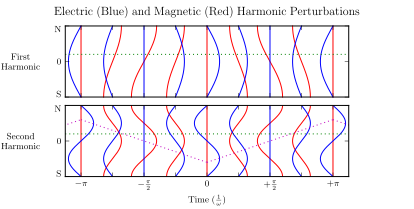
\includegraphics[width=\textwidth]{figures/harmonics.pdf}
    \caption[First and Second Harmonic Resonances]{
      The first (or fundamental) harmonic has an an antinode in its perpendicular electric field (blue) at the equator, along with a node in its perpendicular magnetic field perturbation (red). A single satellite can identify the first harmonic by the relative phase of the electric and magnetic field perturbations: an observer north of the equator (green) will see the electric field perturbation lead the magnetic field by \SI{90}{\degree}. The second harmonic is the opposite: it has an electric field node at the equator, and an observer north of the equator will see the electric field perturbation lag the magnetic field by \SI{90}{\degree}. The purple line sketches the path of a particle in drift-bounce resonance; in the particle's rest frame, the electric field is always to the right. 
    }
    \label{fig_harmonics}
\end{figure}

A first-harmonic FLR that is periodic or localized in the azimuthal direction is conducive to drift-resonant wave-particle interactions\cite{dai_2013,poulter_1983}. The particle is like a child on a swing: whenever the path of the particle (or child) gets close to the wave (parent), it gets a push, and always in the same direction. The wave fields spend half its time pointing the other direction, just as the parent must shift their weight backward to get ready for the next push, but at that point the particle (child) is far away. 

Second-harmonic FLRs interact with particles through the drift-bounce resonance, which is slightly more complicated. As the particle drifts azimuthally, it also zig-zags north-south. The combination of those two periodic motions must align with the phase of the wave electric field. An example path is shown by the purple line in \cref{fig_harmonics}: the particle experiences a rightward electric field throughout the wave's oscillation. 

The drift and drift-bounce resonance conditions is written, respectively\cite{takahashi_2011}:
\begin{align}
  \omega - \azm \omega_D &= 0 &
  &\text{and}&
  \omega - \azm \omega_D &= \omega_B
\end{align}

Where $\omega$ is the frequency of the wave, $\omega_D$ and $\omega_B$ are the particle's drift and bounce frequencies respectively, and \azm is the wave's azimuthal modenumber, as discussed in \cref{sec_azm}. 

In principle, the first and second harmonics can be distinguished by their frequencies, even from a single-point observation\cite{cummings_1969,green_1985}.  In practice, however, this is not a reliable approach\cite{takahashi_2013}. There are significant uncertainties surrounding the number density profile --- and thus the \Alfven speed profile --- along a geomagnetic field line. 

Harmonic structure can also be deduced by noting the phase offset between the wave magnetic field and its electric field (or the plasma velocity)\cite{dai_2015,takahashi_1992}. In \cref{fig_harmonics}, the green line indicates an observer just north of the magnetic equator. For the first harmonic, the observer sees the electric field waveform lead the magnetic field by a phase of \SI{90}{\degree}; for the second harmonic, the electric field waveform lags by \SI{90}{\degree}. (South of the equator, the signs are reversed.) Notably, this approach has only become viable with the advent of satellites carrying both electric and magnetic field instrumentation, such as THEMIS in 2007\cite{angelopoulos_2008} and the Van Allen Probes\footnote{The Van Allen Probes were previously called RBSP, for Radiation Belt Storm Probes. } in 2012\cite{stratton_2012}. 

Strictly speaking, the the phase offset of the electric and magnetic fields does not provide the harmonic number --- only its parity. It's reasonably safe to assume that an even mode is the second harmonic; the second harmonic is by far the most commonly observed\cite{hughes_1978,singer_1982,takahashi_1990}, due in part to its excitement by the antisymmetric balloon instability\cite{chan_1994,chen_1991,cheng_1994,southwood_1976}. However, the distinction between the first and third harmonics is not always clear; this issue is discussed further in \cref{ch_rbsp}. Higher harmonics than that are not expected in the Pc4 frequency band. 

% Of 390 noncompressional events, Dai identified 19 to be clearly fundamental mode and 197 to be clearly second harmonic\cite{dai_2015}. 

\todo{Second-harmonic FLRs are unlikely to cause ground signatures\cite{takahashi_1992}. }

\todo{Dai found a nice event\cite{dai_2013} that was unambiguously determined to be a fundamental-mode Pc4 in drift-resonant interaction with \about\SI{e5}{\eV} ions. Consistent with \cite{thompson_2001}. Other observations of odd harmonics: \cite{yang_2010,eriksson_2005}. }

% -----------------------------------------------------------------------------
% -----------------------------------------------------------------------------
% -----------------------------------------------------------------------------
\section{Azimuthal Modenumber}
  \label{sec_azm}

The wavelength of an FLR in the azimuthal direction is indicated by its azimuthal wavelength. A wave with modenumber \azm has an azimuthal wavelength that spans $\frac{24}{\azm}$ hours in MLT. 

\begin{figure}[!htb]
    \centering
    \includegraphics[width=\textwidth]{figures/placeholder.jpg}
    \caption[Large and Small Azimuthal Modenumbers]{
      \todo{Large and small azimuthal modenumbers.}
    }
    \label{fig_azm}
\end{figure}

Waves with small azimuthal modenumbers ($0 < \azm < 10$) are typically driven by broadband energy sources at the magnetosphere's boundary, such as variations in the solar wind pressure\cite{degeling_2014,hao_2014,kessel_2008,zong_2007,zong_2009}, sporadic magnetic reconnection\cite{hughes_1994}, or Kelvin-Helmholtz waves on the magnetopause\cite{chen_1974,liu_2011,southwood_1974}. In the low-\azm regime, the shear and compressional \Alfven waves are coupled, which allows energy to move across field lines until the driving frequency lines up with the local \Alfven frequency\cite{lysak_1992}. Because of their broadband energy source, low-\azm FLRs often have a mishmash of frequencies present in their spectra\cite{dai_2015}.

When the azimuthal modenumber is large (or, equally, when the azimuthal wavelength is small), the shear and compressional \Alfven waves are decoupled\cite{cummings_1969,radoski_1974}\footnote{Equally, the strength of a wave's parallel component hint at its modenumber, a point which is revisited in \cref{ch_rbsp}. }. As a result, FLRs must be driven from within the magnetosphere. Proposed energy sources include phase space gradients near the plasmapause\cite{dai_2013}, particularly as the plasmasphere refills after a storm or substorm\cite{engebretson_1992,liu_2013}. 

The ionosphere is known to attenuate waves with small spatial extent in the perpendicular direction\cite{hughes_1976,wright_1999,yeoman_2001}. As a result, FLRs may create no signature on the ground if their azimuthal modenumber is large. For example, a recent paper by Takahashi shows a strong (\SI{2}{\nT} at $L\sim10$), clear resonance with $|\azm|\gtrsim70$ and no corresponding ground signature\cite{takahashi_2013}. 

Southwood\cite{southwood_1976} and Glassmeier\cite{glassmeier_1984} show that a low frequency wave passing through the ionosphere on its way to Earth will be attenuated per
\begin{align}
  \label{attenuation}
  \frac{B_E}{B_I} &= \frac{\Sigma_H}{\Sigma_P} \exp \arg{ -\azm \frac{R_I - R_E}{R_E \sin \theta} }
\end{align}

Where $B_E$ and $B_I$ are the magnetic field strengths at $R_E$ (Earth's surface, \SI{6783}{\km} geocentric) and $R_I$ (the ionosphere, \about\SI{6900}{\km} geocentric) respectively. The integrated ionospheric Pedersen and Hall conductivities, $\Sigma_P$ and $\Sigma_H$, are typically within a factor of two of one another. Field lines near the plasmapause can be traced to Earth at $\sin\theta\about0.4$. That is, by the time it reaches the ground, the magnetic field from an FLR with $m=10$ is weaker by a factor of two; at $m=100$, the factor is closer to 100. 

% -----------------------------------------------------------------------------
% -----------------------------------------------------------------------------
% -----------------------------------------------------------------------------
\section{Poloidal and Toroidal Polarizations}

%- One sentence paragraphs aren't
%- "Perhaps not coincidentally" Perhaps?
%- Fig. 3.4: I don't know how to read this plot. I guess the left is the first harmonic and the right is the second, but at first glance they looked the same. I guess I get it now...
%- Page 18 (page number not PDF number): You have half a sentence hanging on. You should probably make this images their own page.

Based on polarization, each FLR can be classified as either poloidal or toroidal. The poloidal mode is a field line displacement in the meridional plane, as shown in \cref{fig_poloidal}, with an accompanying electric field in the azimuthal direction. The toroidal mode's magnetic displacement is azimuthal, per \cref{fig_toroidal}; the associated electric field is in the meridional plane. 

\begin{figure}[!htb]
    \centering
    \includegraphics[width=\textwidth]{figures/poloidal.pdf}
    \caption[Poloidal Mode Structure]{
      The poloidal resonance is a magnetic field in the meridional plane. The displacement is radial near the equator, and can be accompanied by enhancement in the parallel magnetic field near the ionosphere. The first harmonic is shown on the left, and the second harmonic on the right. Lines are colored red and blue only to contrast with the unperturbed black field line. 
    }
    \label{fig_poloidal}
\end{figure}

\begin{figure}[!htb]
    \centering
    \includegraphics[width=\textwidth]{figures/toroidal.pdf}
    \caption[Toroidal Mode Structure]{
      A toroidally-polarized FLR has a magnetic perturbation in the azimuthal direction, as shown. Bold lines are taken to be above the page, and dotted lines below the page, with the displacement indicated by the line's width. The first harmonic --- where the entire field line oscillates in and out of the page --- is shown on the left. The second harmonic is on the right, with northern and southern halves perturbed in opposite directions. 
    }
    \label{fig_toroidal}
\end{figure}

Both poloidal and toroidal waves are noted for their ability to contribute to the energization and radial diffusion of trapped particles. The poloidal mode interacts more strongly, since its electric field is aligned with the trapped particles' drift motion. Poloidally-polarized waves are also more prone to creating magnetic signatures on the ground, due to ducting in the ionosphere\cite{fujita_1988,greifinger_1968}. 

Toroidal modes have been shown to far outnumber poloidal modes\cite{anderson_1990}. Perhaps not coincidentally, poloidally-polarized waves rotate asymptotically to the toroidal mode\cite{mann_1995,mann_1997,radoski_1974}. Poloidal waves with low azimuthal modenumber --- such as those driven by broadband sources at the magnetopause --- rotate on timescales comparable to their oscillation periods. 

\todo{Fishbone instability\cite{chen_1984,mcguire_1983}. Like the poloidal mode, but for lab plasmas. }

\todo{Poloidal and toroidal modes are coupled by the ionospheric Hall conductivity\cite{kato_1956}. The Hall conductivity also increases the ``ringtime'' of these resonances, allowing them to oscillate through the inductive process rather than be dissipated as Joule heating\cite{waters_2013}. }

\todo{Toroidal modes show a clear frequency dependence with $L$. Poloidal modes less so. Citation...? }

% -----------------------------------------------------------------------------
% -----------------------------------------------------------------------------
% -----------------------------------------------------------------------------
\section{Giant Pulsations}

%- What's special about Tromso Norway? I feel like you need half a sentence more!

The study of geomagnetic pulsations long predates satellites, sounding rockets, or even the word ``magnetohydrodynamics''\footnote{The term was first used by \Alfven in the 1940s\cite{alfven_1946}. }. Large, regular oscillations in the magnetic field were noted as early as 1901\cite{birkeland_1901}. Eventually, the term ``giant pulsation,'' or Pg, arose to describe such pulsations. 

On the ground, Pgs are notable for their strikingly sinusoidal waveforms, their eastward drifts, and their specific occurrence pattern: Pgs are typically seen pre-dawn, at latitudes of \SIrange{60}{70}{\degree}. Pgs generally fall into the Pc4 frequency band\footnote{The Pc4 range is periods of \SIrange{45}{140}{\s}, while Pgs are often said to range from \SIrange{60}{200}{\s}\cite{brekke_1987}. }. Their harmonic structure was a source of controversy for decades, but recent multisatellite observations seem to be in agreement that they are odd harmonics, probably fundamental\cite{glassmeier_1999,hillebrand_1982,kokubun_1980,kokubun_1989,takahashi_2011,takahashi_1992}. They are poloidally polarized, with modenumbers $10 \lesssim \azm \lesssim 40$\cite{glassmeier_1980,hillebrand_1982,poulter_1983,rostoker_1979,takahashi_1992}. 

Whereas FLRs are waves in space which may produce ground signatures, ``giant pulsation'' refers to the ground signature specifically\footnote{Historically, the wave designations shown in \cref{tab_iaga} 
all referred to ground phenomena. Over time, they have come to describe satellite observations as well, including those without corresponding signatures on the ground. }. That is, Takahashi's satellite observation of a sinusoidal, morningside, high-\azm, fundamental poloidal resonance was not classified as a Pg because it did not produce a signal on the ground\cite{takahashi_2013}. 

%  --- half of them measured at Troms{\o}, Norway

Due to their remarkably clear waveforms, Pgs are typically found by ``visual inspection of magnetometer data''\cite{motoba_2015}. Over the course of the past century, a number of multi-year (sometimes multi-decade\cite{brekke_1987}) surveys have totaled nearly one thousand Pg events. On average, a ground magnetometer near \SI{66}{\degree} magnetic latitude observes \about10 Pg events per year\cite{brekke_1987,harang_1941,rolf_1931,sucksdorff_1939}. Observations are not distributed uniformly; rather, giant pulsations become more common near the equinox and during times of low solar activity. 

Unlike Pc4 pulsations in general, Pgs show no particular correlation with storm phase\cite{motoba_2015}. However, they do often occur as the magnetosphere recovers from a substorm\cite{motoba_2015,rostoker_1979}. 

% -----------------------------------------------------------------------------
% -----------------------------------------------------------------------------
% -----------------------------------------------------------------------------
\section{Motivations for the Present Work}

A great deal has been learned --- and continues to be learned --- through observations of field line resonance. However, the cost-to-benefit ratio is climbing. As summarized in the sections above, FLR behavior depends significantly on harmonic structure, azimuthal modenumber, and polarization --- not to mention frequency, spectral width, and so on. With each degree of freedom comes the necessity for an additional simultaneous observation. 

Similarly, as FLRs have been shown to depend on ever-more-specific magnetospheric conditions, analytical techniques have fallen out of favor. The height-resolved ionosphere, the multidimensional \Alfven speed profile, and the inconvenient geometry combine to create a problem beyond the reasonable purview of pencil and paper. 

That is, the topic of field line resonance is ripe for numerical modeling. 

Past models of the magnetosphere have been ill-suited for the consideration of FLRs. Reasons include overly-simplified treatment of the ionospheric boundary, no consideration of the plasmapause, limited range in \azm, and the inability to compute ground signatures. \cref{ch_model} presents a model which addresses these issues, allowing the computation of field line resonance with unparalleled attention to realism. 

The model allows a bird's-eye view of the structure and evolution of FLRs. As such, not only can several open questions be addressed, but their answers serve to unify a number of seemingly-disparate properties described in the sections above. 

The rotation of poloidally-polarized waves to the toroidal mode is investigated. Particular attention is paid to the importance of azimuthal modenumber and ionospheric conductivity. The interplay between said rotation and the transport of energy across field lines --- which also depends on azimuthal modenumber --- is considered as well. 

By their nature, drifting particles have the potential to spur wave-particle interactions at all MLT. However, Pc4 observations are strongly peaked on the dayside. In a 2015 paper, Dai notes, ``It is not clear why noncompressional [high-\azm] Pc4 poloidal waves, which are presumably driven by instability within the magnetosphere, preferrentially occur on the dayside''\cite{dai_2015}. Motoba, later that year, echoes, ``It is unclear whether other generation mechanisms of fundamental standing waves ... can explain the localization of Pgs in local time''\cite{motoba_2015}. This, too, is considered numerically: to what degree is field line resonance affected by the (day-night asymmetric) conditions of the ionosphere? 

\todo{Transition... With the above in mind, what data would be super helpful? }

It's been shown that a ground magnetometer \SI{66}{\degree} north of the magnetic equator observes \about10 Pg events per year. It's also been shown that poloidal Pc4s are rare compared to toroidal ones, and that most poloidal Pc4s are even harmonics. However, little attention has been paid to how these rates line up with one another. Given the relative occurrence rate of poloidal and toroidal waves, of odd and even harmonics, and of diffuse and sharp spectral peaks, just how unusual are giant pulsations? 


%The present work uses a numerical model to investigate the preferrential occurrence of field line resonances in the Pc4 range --- particularly first-harmonic poloidal modes, such as giant pulsations --- in MLT. 

%Giant pulsations are commonly referred to as ``rare''\cite{brekke_1987}, or even ``a small subset of fundamental poloidal waves''\cite{takahashi_2013}. However, quantification of Pg occurrence --- compared to the occurrence rate of fundamental poloidal Pc4s in general --- is thin on the ground. It's been shown that poloidal Pc4s are rare compared to their toroidal counterparts. It's also been shown that, among poloidal Pc4s, the second harmonic is the most common. 


% Dai writes, in his 2015 paper\cite{dai_2015}, ``It is not clear why noncompressional [high-\azm] Pc4 poloidal waves, which are presumably driven by instability within the magnetosphere, preferrentially occur on the dayside.'' 

% Motoba\cite{motoba_2015}, similarly, notes ``It is unclear whether other generation mechanisms of fundamental standing waves ... can explain the localization of Pgs in local time.''


% Giant pulsations have variously been referred to as ``intriguing''\cite{green_1985}. ``rare''\cite{brekke_1987}, even to the point of being ``a small subset of fundamental poloidal waves''\cite{takahashi_2013} --- note that it's well known that fundamental poloidal mode waves are already rare in comparison to second harmonic waves. 


%\todo{What's going on with the MLT localization of Pc4 pulsations? Is there something spooky going on with the driving? Maybe the ionosphere just kills FLRs on the nightside! }

%\todo{What's so special about Pgs? How rare are they, really, compared to fundamental poloidal modes in general? How does that line up with the occurrence rate of nice, sinusoidal waveforms in second-harmonic Pc4s? That is, is there something special about Pgs, or do they just live in a ``sweet spot'' with respect to constraints on observation and resonance? }

%\todo{Parallel electric fields. In this regime, we're looking at inertial effects, not kinetic effects\cite{goertz_1979,thompson_1996}. Should produce non-monoenergetic precipitation, which are observed\cite{goertz_1984}. Consistent with MHD models\cite{chaston_2000,chaston_2002}. Inertial-scale structures observed with Polar\cite{wygant_2002}. }

%\todo{The plasmapause matters! Effective potential well, analogous to \Schrodinger's equation\cite{lee_1998,lee_1999,dai_2009}. Shown in theory\cite{klimushkin_1998,leonovich_2000,klimushkin_2004,mager_2013} and in observation\cite{takahashi_2009,takahashi_2010}.  }

%\todo{All sorts of FLR occur preferrentially (though not exclusively) on the dayside\cite{dai_2015,ukhorskiy_2005}. }

%\todo{Any waves with frequencies of $\SIrange{e-3}{1}{\Hz}$ are termed ULF waves --- ultra low frequency. ULF waves are furthermore categorized in terms of their morphological characteristics. Pc waves are continuous (exhibiting a fairly consistent waveform over a large number of wave periods) while Pi are irregular; the waves are further partitioned into frequency bands. See \cref{tab_iaga}. }

%\todo{These are Jacobs' original ranges... but are they really reflective of the jargon still used? It's weird that these ranges bottom out so far below 1000s. }

%\todo{While the IAGA characterizations are based on wave morphology, they do a decent job of deliniating between the different underlying physical processes as well. Pi2 pulsations (irregular waves with periods of a minute or two) tend to be excited on the nightside; they are associated with substorm onset (though the processes that give rise to Pi2s --- and their relation to substorm onset --- remains controversial). Pc1 and Pc2 pulsations tend to be EMIC (electromagnetic ion cyclotron) waves near the ion gyrofrequency, which are important for the precipitation of electrons (?). }

%Pi2: ``Clearly linked to substorm disturbances and other impulsive dynamics are the irregularly shaped waves in the 7--25-mHz band referred to as Pi2. Recent work on these waves suggests that their periodicity reflects the spectrum of global mode excitations of the plasmasphere but there is a competing proposal that the dominant frequencies are imposed by the modulated flows in the magnetotail.''\cite{kivelson_2006}

%\todo{The present work is specifically concerned with field line resonances near the plasmapause. These waves fall in the Pc4 range, with frequencies around \SI{10}{\mHz}\footnote{Notably, field line resonances can also fall within the Pc3 and Pc5 ranges. }. }

% Less than a decade later, Sigura presented observational evidence of the phenomenon: a wave seen simultaneously at the northern and southern foot points of a geomagnetic field line\cite{sigura_1961}. 

%\todo{There's no discussion of ULF frequency bands, or even use the term ``Pc4.'' That's probably a problem. Introduce \SIrange{7}{25}{\mHz}! }

% \todo{Pc4s are localized in L and in MLT\cite{anderson_1990,dai_2015,engebretson_1992,liu_2009}. Near the plasmapause. This is an important part of why the 2.5D model is a good fit! }

% \todo{Drift resonance with azimuthal wavenumber. In the analogy of a parent pushing a child on the swing, the child still gains energy even if the parent only shows up half the time. Or Are there a bunch of parents? The analogy starts to fall apart past there. }

%``To summarize, the general buffetting of the magnetosphere by variations in the solar wind dynamic pressure, or perhaps by sporadic magnetic reconnection, provides a broad band energy source to the magnetosphere. The magnetospheric cavity as a whole rings at its own eigenfrequencies, thus transporting energy at just those frequencies to field lines deep in the magnetosphere. Those field lines whose eigenfrequencies match one of the cavity eigenfrequencies couple to the cavity mode and resonate strongly, producing the classical field line resonance signature.\cite{hughes_1994}'' 

% Compressional driving doesn't preclude drift or drift-bounce resonance\cite{zong_2007,zong_2009}. 

% The strength of the compressional-poloidal coupling indicates \azm\cite{hughes_1994}. 

% Low-\azm waves tend to be more muddled... driven by broadband sources rather than resonance\cite{dai_2015}. 

% Small structures are also damped; resonances narrower than $\sim \SI{100}{km}$ aren't visible on the ground. See also Glassmeier and Stellmacher, 2000 (about small latitude). \Alfven waves with small latitudinal scale\cite{glassmeier_2000} are screened by the ionosphere. Attenuation factor from \cite{hughes_1976} and \cite{glassmeier_1984}. 

%``Pgs maybe a manifestation of a small subset of fundamental poloidal waves excited in the magnetopause.'' \cite{takahashi_2013}

%``It is not clear why noncompressional [high-\azm] Pc4 poloidal waves, which are presumably driven by instability within the magnetosphere, preferrentially occur on the dayside.\cite{dai_2015}''

%``It is unclear whether other generation mechanisms of fundamental standing waves such as drift wave instability\cite{green_1979} can explain the localization of Pgs in local time (LT).''\cite{motoba_2015}

% Shear mode incident on the ionosphere, pederson current closes FAC, Hall current then generates a fast mode wave which may be detected in space or on the ground\cite{tamao_1965}. 

% Poloidal and toroidal ULF polarizations are treated differently by the ionosphere\cite{greifinger_1968} (more recently, \cite{fujita_1988}) due to ducting by the ionosphere. 

% In the example shown of a fundamental mode poloidal Pc4, and in the example of a higher harmonic Pc4, a mishmash of toroidal activity is present. \cite{dai_2015}, figure 8 and 9 respectively. 

% Observations of odd-mode poloidal waves... possible fundamental\cite{yang_2010,eriksson_2005}.

% \todo{Do the unambiguous Pc4 events in \cite{takahashi_2011} and \cite{dai_2013} also have a mishmash of toroidal activity? NO. }

% Poloidal Pc4s occur primarily during geomagnetically active times\cite{dai_2015}. This confirmed and refined older work\cite{engebretson_1987}. 

% Drift resonance happens when the bounce frequency of an \Alfven wave between the northern and southern ionospheres matches the bounce frequency of nearby particles. It allows the energization of ring current and radiation belt particles through drift and drift-bounce resonance\cite{elkington_1999,mann_2013,ozeke_2008,southwood_1976}. By multiple wave-particle interactions, poloidal ULF waves [FLRs] can lead to radial diffusion of radiation belt particles\cite{elkington_2003,ozeke_2012,tu_2012}.

%\begin{figure}[!htb]
%    \centering
%    \includegraphics[width=\textwidth]{figures/fa.pdf}
%    \caption[\Alfven Bounce Frequency Profiles]{
%      \Alfven bounce frequency profiles, computed by integrating the the \Alfven speed back and forth over a field line. $f_A = \lrb{ \oint \frac{dz}{v_A} }^{-1}$. Dotted lines indicate the Pc4 frequency range, \SIrange{7}{25}{\mHz}. In each profile, the effect of the plasmapause is clearly visible, centered at $L=4$. Field lines just inside and just outside the plasmapause appear susceptible to resonance in the Pc4 band. \todo{Talk about how the size of the plasmasphere can be adjusted, and \SI{4}{\RE} is just a typical value. }
%    }
%    \label{fig_fa}
%\end{figure}

% ULF waves have been shown to correlate with pulsating aurora and with chorus\cite{jaynes_2015}. It's believed that (in the case presented) substorm injection drove Pc4-5 pulsations, which modulated chorus waves, which pitch-angle scattered electrons with energies on the order of \SI{10}{\kilo\eV}. 

% \todo{Theoretical consideration of decay vs propagation, by frequency. Lysak and Yoshikawa 2006. }

% Drift-wave instability\cite{hasegawa_1971,green_1979,green_1985} is also a possibility for exciting fundamental poloidal waves, though it requires cold plasma, so it could only happen in the plasmasphere. 

% AMPTE/CCE data has shown a correlation between poloidal Pc4 activity and intense ring current flux near the equator\cite{engebretson_1988}. 

% Toroidal mode is usually associated with external driving\cite{chen_1974,southwood_1974}. 

% A Hall-conducting ionosphere reflects ULF waves\cite{hughes_1974}. 

% Compressional poloidal Pc4 pulsations are much more common during storms, but not particularly sensitive to storm phase. Noncompressional ones occur primarily during recovery\cite{dai_2015,rostoker_1979,engebretson_1992,anderson_1994}. Note that Dai\cite{dai_2015} was pretty generous about what counted as a storm... anything that hits \SI{-30}{\nano\tesla}. So \cite{motoba_2015} may not have counted the same way when they found no particular correlation with storm phase. 

%\todo{First Pg observation\cite{birkeland_1901}. }

%\todo{Strong poloidal (that is, meridional) polarization in space, combined with the \about\SI{90}{\degree} rotation of long-period waves by the ionosphere\cite{nishida_1964_screening,hughes_1974}, gives Pgs a distinctive east-west polarization on the ground. }

%\todo{Pgs are most common during solar minimum, perhaps because of decreased mass loading of heavy ions\cite{denton_2011}. }

%\todo{The harmonic structure of giant pulsations was once controversial; at this point, there is general consensus (based on satellite data) that they are fundamental poloidal modes\cite{glassmeier_1999,hillebrand_1982,kokubun_1980,kokubun_1989,takahashi_1992,takahashi_2011}. }

%\todo{Giant pulsations observed on the ground tend to have azimuthal modenumbers $10 \lesssim \azm \lesssim 40$\cite{glassmeier_1980,hillebrand_1982,poulter_1983,rostoker_1979,takahashi_1992}. }

%\todo{Giant pulsations peak around \SI{66}{\degree} MLAT\cite{motoba_2015}, corresponding to L=6, but have been observed at $5 \lesssim L \lesssim 7$\cite{green_1985}. Most prevalent on the morningside, with some in the afternoon. }

% Another past study: \cite{takahashi_1984_spectrum}. Satellite data is surveyed and classified by polarization, harmonic, wavenumber, etc, in order to determine the mechanisms for generating \Alfven waves. Old, but still pretty representative, according to Motoba\cite{motoba_2015}. 

% A long-period \Alfven wave passing through the ionosphere is rotated by about 90 degrees\cite{nishida_1964_screening,hughes_1974}. That would translate a poloidal resonance in space to an east-west ground signature. 

% \cite{motoba_2015} suggests that Pgs originate from the fundamental poloidal mode waves at all local times. 

% It seems to be the convention to find a Pg event on the ground, then look at satellite data. That's certainly what was done in \cite{motoba_2015}. 

% Per \cite{motoba_2015}, most Pg events happen around $L=7$, but some do happen near the plasmapause, as seen(?) by \cite{green_1985}. 

% ``The AL distribution shown in Figure 14c are consistent with the findings of \cite{rostoker_1979} that Pgs occur as the magnetosphere recovers from previous activities (substorms).''\cite{motoba_2015} Finds this to be reasonable because it's ``very likely'' that energetic ions injected into the inner magnetosphere from the magnetotail provide energy to Pgs. 

% Analysis of GOES data from 2008 to 2013 shows about 100 Pg events. They are concentrated on the morningside. No particular correlation with storm phase\cite{motoba_2015}. 

% Recall compressional poloidal Pc4s are mostly during storm time, and noncompressional are mostly specifically during late recovery\cite{dai_2015}. Only 19 fundamental poloidal mode examples were identified from the 390 noncompressional poloidal events. 

%
% From W J Hughes' Magnetospheric ULF Waves: A Tutorial With a Historical Perspective
%

% rolf 1920 for early observation of Pi2

% Patel 1965 made observations in space, and matched them to observations on the ground
% Cummings et al 1969 numerically integrated Dungey's equations to estimate eigenfrequencies
% soviets discovered that different pulsations have different sources in the 1970s; see troitskaya 1993 and greenstadt and russell 1993
% troitskaya 1969 showed that Pc3 can sometimes be explained by a sudden change in the size of the magnetosphere following an impulse. an example --- this must have also been seen earlier. because... 
% Bolshakova and Troitskaya 1968 showed that Pc3 observation depends on IMF N/S. Iff IMF is within about 50 degrees of the earth-sun linem Pc3 is observable on the ground. 
% Troitskaya et al 1971 showed Pc3 frequencies at L=3 depend on IMF magnitude
% Gul'elmi 1974 and Kovner et al gave theoretical justification for these observations. 
% Russell and Hoppe 1981 made observations upstream of the bow shock to unify some ideas. upstream waves are driven by ion cyclotron instability, which depends on IMF magnitude. 

% Gringauz et al 1970 found that solar wind number density affects Pc3 and Pc4 periods (oppositely). The Pc4 effect is a standing question. 

% Samson et al 1971 new observations with digital recording and arrays near the plasmapause! they showed MLT dependence of peak amplitude, and different regions of opposite circular polarization. 
% Dungey 1954 had suggested KH as a wave energy source, which explained the flipping circular polarization at noon. 
% Southwood 1974 went back to the equations and came up with a reason for resonance. waves hitting the bow shock propagate in as an evanescent fast mode. when it gets to a resonant field line, the fast mode couples to the shear mode. the energy tunnels. this only happens if dissipation is finite. 
% Chen and Hasegawa 1974 did too, independently
% Newton et al 1978 showed that joule dissipation at the ionosphere is dominant, and that the amount of dissipation determines the width of the resonance. 

% kivelson et al 1984 argued for cavity mode eigenfrequencies. Pc5. 
% kivelson and southwood 1985, 1986 did analytical work to defend it. 
% Lee and Lysak 1991 did numerical work in a dipole geometry. 

% Harrold and Samson 1992 The waves probably have to be reflected by the bow shock, not by the magnetopause, to line up with the observed eigenfrequencies. 1 to 3 mHz. 

% allan et al 1985 did early observation of ULF waves (Pc5 and Pc4) from waveform plots. 
% Waters et al 1991 ground-based observation of Pc3 and Pc4 before spacecraft existed at small L. 
% Menk et al 1993 also









%\begingroup\let\clearpage\relax
% put sections that make up a chapter here to prevent newpage between sections.
%\endgroup
%\newpage

%\begingroup\let\clearpage\relax
% %%%%%%%%%%%%%%%%%%%%%%%%%%%%%%%%%%%%%%%%%%%%%%%%%%%%%%%%%%%%%%%%%%%%%%%%%%%%%
% %%%%%%%%%%%%%%%%%%%%%%%%%%%%%%%%%%%%%%%%%%%%%% Description of Numerical Model
% %%%%%%%%%%%%%%%%%%%%%%%%%%%%%%%%%%%%%%%%%%%%%%%%%%%%%%%%%%%%%%%%%%%%%%%%%%%%%

\chapter{Model}
  \label{ch_model}

\todo{This chapter runs through the numerical model... starting with the math that underlies it, then looking at the model itself, then a cool extra thing. }







``Increasing the Hall conductance allows the energy to oscillate through the inductive process rather than dissipate as Joule heating, increasing the `ringtime' of field line resonances.''\cite{waters_2013}



Ionospheric profiles are static for the duration of a simulation. Even so-called ultra low frequency waves are still much faster than convective timescales. Each profile is resolved to an altitude of about $\SI{e4}{\km}$, and include well-resolved $E$, $F_1$, and $F_2$ layers. 


  % =============================================================================
% =============================================================================
% =============================================================================
\section{Dispersion Relation}
  \label{sec_math}

Before delving into the implementation of the numerical model, it's instructive to consider the fundamental equations of waves in a cold, resistive plasma. 

The evolution of electric and magnetic fields is governed by \amplaw and \farlaw. Notably, the present work takes the linearized versions of Maxwell's equations; the vectors \vec{E} and \vec{B} indicate perturbations above the zeroth-order magnetic field. 
\begin{align}
  \label{math_maxwells}
  \tensor{\epsilon} \cdot \ddt \vec{E} &= \oomz \curl{B} - \vec{J} & \ddt \vec{B} &= -\curl{E}
\end{align}

Current follows \ohmlaw. For currents perpendicular to the background magnetic field, Kirchhoff's formulation is sufficient. Conductivity is much higher along the magnetic field lines\footnote{The dipole coordinate system is defined rigorously in \cref{sec_coords}; at present, it's sufficient to take \zhat parallel to the zeroth-order magnetic field, and \xhat and \yhat perpendicular to \zhat (and to each other). }, so it's appropriate to also include the electron inertial term\footnote{Electron inertial effects are not included in the model described in \cref{sec_tuna}, or in the results in \cref{ch_results}; however, their implementation and impact are explored in \cref{sec_inertia}. }. 
\begin{align}
  \label{math_ohms}
  0 &= \tensor{\sigma}_\bot \cdot \vec{E}_\bot - \vec{J}_\bot &
  \frac{\me}{n e^2} \ddt J_z &= \sz E_z - J_z
\end{align}

The derivatives in \cref{math_maxwells,math_ohms} can be evaluated by performing a Fourier transform. They can then be combined, eliminating the magnetic field and current terms. 
\begin{align}
  \label{disp_setup}
\begin{alignedat}{4}
  & 0 = \vec{E}_\bot && + \frac{\va^2}{\omega^2} \lr{ \vec{k} \times \vec{k} \times \vec{E} }_\bot && + \frac{i}{\ep \omega} \tensor{\sigma}_\bot \cdot && \vec{E}_\bot \\
  & 0 = E_z && + \frac{c^2}{\omega^2} \lr{ \vec{k} \times \vec{k} \times \vec{E} }_z && + \frac{i \op^2 }{\omega \lr{\nu - i \omega} } && E_z
\end{alignedat}
\end{align}

The speed of light, \Alfven speed (including the displacement current correction), plasma frequency, and parallel conductivity are defined in the usual way: 
\begin{align}
  \label{def_basics}
  c^2 & \equiv \frac{1}{\mz \ez} &
  \va^2 & \equiv \frac{1}{\mz \ep} &
  \op^2 & \equiv \frac{n e^2}{\me \ez} &
  \sz & \equiv \frac{n e^2}{\me \nu}
\end{align}

Using the vector identity $\vec{k} \times \vec{k} \times \vec{E} = \vec{k} \, \vec{k} \cdot \vec{E} - k^2 \vec{E}$, \cref{disp_setup} can be reassembled into a single expression, 
\begin{align}
  \label{disp}
  0 &= \lr{ \tensor{ \mathbb{I} } + \frac{1}{\omega^2} \tensor{V}^2 \cdot \vec{k} \, \vec{k} - \frac{k^2}{\omega^2} \tensor{V}^2 + \frac{i}{\omega} \tensor{\Omega} } \cdot \vec{E}
\end{align}

Where $\tensor{ \mathbb{I} }$ is the identity tensor and in \x-\y-\z coordinates\footnote{Note that the present definition of \tensor{\Omega} differs slightly from that used in \cref{sec_eqns}. }, 
\begin{align}
  \tensor{V}^2 &\equiv 
    \mmm{\va^2}{0}{0}
        {0}{\va^2}{0}
        {0}{0}{c^2} &
  & \text{and} &
  \tensor{\Omega} &\equiv 
    \mmm{ \frac{\sp}{\ep} }{ \frac{-\sh}{\ep} }{0}
        { \frac{\sh}{\ep} }{ \frac{\sp}{\ep} }{0}
        {0}{0}{ \frac{\op^2}{\lr{\nu - i \omega}} } 
\end{align}

In \cref{disp}, the expression in parentheses is the dispersion tensor. Nontrivial solutions exist only when its determinant is zero. This gives rise to a seventh-order polynomial in $\omega$, so rather than a direct solution it's necessary to consider limits of specific interest. 

% -----------------------------------------------------------------------------
% -----------------------------------------------------------------------------
% -----------------------------------------------------------------------------
\subsection{Parallel Propagation}
  \label{sec_par}

\todo{Parallel propation -- \vec{k} aligned exactly with \zhat -- is a cartoon version of field line resonance. }

In the parallel propagation limit, the wave vector \vec{k} is taken to lie along the \z axis. In that case, the parallel and perpendicular components of the determinant of the dispersion tensor are decoupled, and can be considered separately. 

The parallel-polarized term gives
\begin{align}
  % Parallel propagation, parallel polarization. 
  0 &= \omega^2 + i \nu \omega - \op^2 &
  & \text{so} &
  a &= b
\end{align}

This expression can be solved directly, though it's more informative when expanded in large $\op$. 

\todo{Write out intermediate step. }

Both expressions in \cref{parallel_math_setup} can be solved directly, though the solution to the (cubic) perpendicular propagation case is too long to be useful. After expanding with respect to a very large plasma frequency, the solutions can be written (for parallel and perpendicular propagation respectively): 
\begin{align}
  % Parallel propagation, parallel polarization. 
  \omega^2 & = \op^2 - i \nu \op + ... \\
\end{align}

The first expression in \cref{parallel_math_final} -- describing the parallel-polarized component of a parallel-propagating wave -- doesn't describe a wave at all; there's no dependence on the wave vector $k$. Instead, it describes the plasma oscillation. The second expression is the O mode: a compressional wave, oscillating just above the plasma frequency, with a parallel electric field. 

The perpendicular factors of the dispersion tensor's determinant, in the cases of parallel and perpendicular propagation respectively, are: 
\begin{align}
  % Parallel propagation, perpendicular polarization. 
  0 &= \omega^4 + 2 i \frac{\sp}{\ep} \omega^3
  - \lr{ 2 k^2 \va^2 + \frac{\sp^2 + \sh^2}{\ep^2} } \omega^2
  - 2 i k^2 \va^2 \frac{\sp}{\ep} \omega
  + k^4 \va^4 \\
\end{align}

First expression of \cref{perpendicular_math_setup} can be solved directly. Noting that $\pm$ and $\opm$ are independent,
\begin{align}
  % Parallel propagation, perpendicular polarization. 
  \omega = \lr{ \frac{\pm \sh - i \sp}{2 \ep} } \opm \sqrt{ k^2 \va^2 + \lr{ \frac{\pm \sh - i \sp}{2 \ep} }^2 }
\end{align}

This wave is propagating along the field line, so the Pedersen and Hall conductivities are small for the vast majority of its trajectory. Expanding, then, gives
\begin{align}
  % Parallel propagation, perpendicular polarization. 
  \omega^2 = k^2 \va^2 \opm k \va \frac{\sh \pm i \sp}{\ep} + ...
\end{align}











... \\ \\ \\






% -----------------------------------------------------------------------------
% -----------------------------------------------------------------------------
% -----------------------------------------------------------------------------
\subsection{Parallel or Perpendicular Propagation}
  \label{sec_par_perp}

\todo{Parallel propagation is ineresting because it's a naive representation of a field line resonance. Perpendicular propagation is interesting because the movement of energy across field lines is a topic of particular interest. In both cases, the cross terms in $\vec{k} \, \vec{k}$ vanish, decoupling the parallel and perpendicular polarizations. }

\todo{Without loss of generality, the wave vector $\vec{k}$ is presumed to lie in the \x-\z plane. The distinction between the azimuthal and crosswise directions is revisited later. }

\todo{ACTUALLY: does this even matter? If we keep $\phi$ in there in addition to $\theta$, does it cancel out? Seems like it should. }

%\subsection{Parallel Polarization}

In the parallel and perpendicular propagation limits respectively, the parallel factors of the determinants of \dispersiontensor are:
\begin{align}
  \label{parallel_math_setup}
  \begin{split}
  % Parallel propagation, parallel polarization. 
  0 &= \omega^2 + i \nu \omega - \op^2 \\
  % Perpendicular propagation, parallel polarization. 
  0 &= \omega^3 + i \nu \omega^2
  - \lr{ k^2 c^2 + \op^2 } \omega
  - i k^2 c^2 \nu
  \end{split}
\end{align}

Both expressions in \cref{parallel_math_setup} can be solved directly, though the solution to the (cubic) perpendicular propagation case is too long to be useful. After expanding with respect to a very large plasma frequency, the solutions can be written (for parallel and perpendicular propagation respectively): 
\begin{align}
  \label{parallel_math_final}
  \begin{split}
  % Parallel propagation, parallel polarization. 
  \omega^2 & = \op^2 - i \nu \op + ... \\
  % Perpendicular propagation, parallel polarization. 
  \omega^2 & = k^2 c^2 + \op^2 - i \nu \op + ...
  \end{split}
\end{align}

The first expression in \cref{parallel_math_final} -- describing the parallel-polarized component of a parallel-propagating wave -- doesn't describe a wave at all; there's no dependence on the wave vector $k$. Instead, it describes the plasma oscillation. The second expression is the O mode: a compressional wave, oscillating just above the plasma frequency, with a parallel electric field. 

The perpendicular factors of the dispersion tensor's determinant, in the cases of parallel and perpendicular propagation respectively, are: 
\begin{align}
  \label{perpendicular_math_setup}
  \begin{split}
  % Parallel propagation, perpendicular polarization. 
  0 &= \omega^4 + 2 i \frac{\sp}{\ep} \omega^3
  - \lr{ 2 k^2 \va^2 + \frac{\sp^2 + \sh^2}{\ep^2} } \omega^2
  - 2 i k^2 \va^2 \frac{\sp}{\ep} \omega
  + k^4 \va^4 \\
  % Perpendicular propagation, perpendicular polarization. 
  0 &= \omega^3 + 2 i \frac{\sp}{\ep} \omega^2
  - \lr{ 2 k^2 \va^2 + \frac{\sp^2 + \sh^2}{\ep^2} } \omega
   - i k^2 \va^2 \frac{\sp}{\ep}
  \end{split}
\end{align}

First expression of \cref{perpendicular_math_setup} can be solved directly. Noting that $\pm$ and $\opm$ are independent,
\begin{align}
  % Parallel propagation, perpendicular polarization. 
  \omega = \lr{ \frac{\pm \sh - i \sp}{2 \ep} } \opm \sqrt{ k^2 \va^2 + \lr{ \frac{\pm \sh - i \sp}{2 \ep} }^2 }
\end{align}

This wave is propagating along the field line, so the Pedersen and Hall conductivities are small for the vast majority of its trajectory. Expanding, then, gives
\begin{align}
  \label{perp_final_z}
  % Parallel propagation, perpendicular polarization. 
  \omega^2 = k^2 \va^2 \opm k \va \frac{\sh \pm i \sp}{\ep} + ...
\end{align}

The second expression of \cref{perpendicular_math_setup} can also be solved directly, though its roots are impractically long. They are expanded with respect to small conductivities (as would be seen by a perpendicular-propagating wave at high altitude) and at large conductivity (representing the perpendicular-propagating wave within the ionosphere). Respectively, 
\begin{align}
  \label{perp_final_x}
  \begin{split}
  % Perpendicular propagation, perpendicular polarization. Small conductivity. 
  \omega^2 & = k^2 \va^2 \pm i k \va \frac{\sp}{\ep} + ... \\
  % Perpendicular propagation, perpendicular polarization. Large conductivity. 
  \omega^2 & = k^2 \va^2 + \lr{ \frac{\sh \pm i \sp}{\ep} }^2 + ...
  \end{split}
\end{align}

\cref{perp_final_z,perp_final_x} describe \Alfven waves: waves traveling at the \Alfven speed (shifted by the ionospheric conductivity) with electric fields perturbations perpendicular to the zeroth-order magnetic field.  

% -----------------------------------------------------------------------------
% -----------------------------------------------------------------------------
% -----------------------------------------------------------------------------
\subsection{High Altitude Limit}
  \label{sec_high_alt}

In the limit of large radial distance, where the density is very low, it's reasonable to neglect the Pedersen conductivity, the Hall conductivity, and the collision rate. 

Without loss of generality, the wave vector $\vec{k}$ can be presumed to lie in the \x-\z plane\footnote{\todo{The azimuthal-propagation case is discussed in XXX.}}. 

Whereas in \cref{sec_par_perp} the parallel component of the determinant of the dispersion tensor could be factored out, the high altitude limit decouples the azimuthal component from those in the meridional plane. The azimuthal component gives, simply, 
\begin{align}
  \omega^2 & = k^2 \va^2
\end{align}

This solution is analogous to the results in \cref{sec_par_perp}: a wave propagating at the \Alfven speed, with electric field perturbation perpendicular to both the zeroth-order magnetic field and the wave vector. 

The meridional components of the determinant of the high-altitude limit of the dispersion tensor give: 
\begin{align}
  \label{high_meridional_setup}
  0 &= \omega^4 
  - \lr{ k_\parallel^2 \va^2 + k_\bot^2 c^2 + \op^2 } \omega^2
  + k_\parallel^2 \va^2 \op^2
\end{align}

Where $k_\parallel$ and $k_\bot$ are the parallel and crosswise components of the wave vector. The a

\cref{high_meridional_setup} is quadratic in $\omega^2$. Its solution is
\begin{align}
  \omega^2 & = \frac{1}{2} \lr{ k_\parallel^2 \va^2 + k_\bot^2 c^2 + \op^2 }
  \pm \sqrt{ \frac{1}{4} \lr{ k_\parallel^2 \va^2 + k_\bot^2 c^2 + \op^2 }^2 
    - k_\parallel^2 \va^2 \op^2 }
\end{align}

Noting that $\op$ is very large, the two roots simplify to
\begin{align}
  \label{high_meridional_final}
  \begin{split}
  \omega^2 & = k_\parallel^2 \va^2 + ... \\
  \omega^2 & = k_\parallel^2 \va^2 + k_\bot^2 c^2 + \op^2 + ...
  \end{split}
\end{align}

\todo{The first part looks like an \Alfven wave. The second is faster than the plasma frequency, so we don't really care about it. }

% -----------------------------------------------------------------------------
% -----------------------------------------------------------------------------
% -----------------------------------------------------------------------------
\subsection{Something Something Implications}
  \label{sec_implications}

\todo{High \azm limit. }

\todo{Hall conductivity? }

\todo{Waves moving at the \Alfven speed constrain time step. }



The electron inertial length $\frac{c}{\op}$ is on the order of \SI{1}{\km}, smaller than the wavelength of a field line resonance by three or four orders of magnitude. That is, at high altitude, the parallel electric field is expected to be smaller than the perpendicular electric field by a factor of \num{e7} -- perhaps more, depending on how closely the wave vector is aligned to the magnetic field. That seems fine -- note that \cref{fig_electric_field_snapshots} shows that max $E_\parallel$ is 4 to 5 orders larger than max $E_\bot$... plus high altitude is the parallel field's minimum and the perpendicular field's maximum. 



With a bit of algebra, the meridional components of the dispersion tensor from \cref{sec_high_alt} provide a comparison of the parallel and perpendicular electric field magnitudes.
\begin{align}
  \frac{E_\parallel}{E_\bot} &= \frac{- k_\parallel k_\bot c^2 }{ \omega^2 - k_\bot^2 c^2 - \op^2 } \sim \frac{k^2 c^2 }{\op^2}
\end{align}










  \include{chapters/sec_tuna}
  % =============================================================================
% =============================================================================
% =============================================================================
\section{Electron Inertial Effects}
  \label{sec_inertia}

As laid out in \cref{sec_tuna}, Tuna resolves neither parallel currents nor parallel electric fields. This limits the model's applicability to \todo{direct acceleration of particles? double layers? \Alfven{}ic aurorae? } and other topics closely related to field line resonance. 

Parallel currents and electric fields can be added to Tuna through the consideration of electron inertial effects in \ohmlaw:
\begin{align}
  0 &= \sz E_z - J_z & \text{becomes} & & \frac{1}{\nu} \ddt J_z &= \sz E_z - J_z
\end{align}

With the addition of the electron inertial term, it is necessary to track the parallel current independent of the parallel electric field\footnote{The parallel current $J_z$ is defined on the same points of the Yee grid as $E_z$. It is offset in time by half of a time step. }. Solving by integrating factors\footnote{The integrating factors technique is laid out explicitly for \amplaw in \cref{sec_eqns}. } gives
\begin{align}
  J_3 &\assign J_3 \, \exp \arg{ - \nu \dt } + \dt \, \frac{n e^2}{\me} E_3 \, \exp \arg{ -\nu \tfrac{\dt}{2} }
\end{align}

From there, the parallel electric field can be updated directly; \cref{e3_final} is replaced by the following: 
\begin{align}
  E_3 &\assign E_3 + c^2 \dt \, \lr{ g_{31} F^1 + g_{33} F^3 } - \frac{\dt}{\ez} J_3
\end{align}

The present section explores the complications that arise from the addition of the electron inertial term to \ohmlaw, as well as a few results that may be gleaned despite those complications. Notably -- for reasons discussed in \cref{sec_lengths} -- the results presented in \cref{ch_results} do not make use of the electron inertial term. 

% -----------------------------------------------------------------------------
% -----------------------------------------------------------------------------
% -----------------------------------------------------------------------------
\subsection{The Boris Factor}
  \label{sec_boris}

With the addition of the electron inertial term, a cyclical dependence appears between \amplaw and \ohmlaw:
\begin{align}
  \ddt E_z &\sim -\frac{1}{\ez} J_z &
  & \text{and} & 
  \ddt J_z &\sim \frac{n e^2}{\me} E_z &
  & \text{so} &
  \frac{ \partial^2 }{ \partial t^2 } E_z &\sim -\op^2 E_z
\end{align}

That is, electron inertial effects come hand in hand with the plasma oscillation. 

\begin{figure}[!htb]
    \centering
    \includegraphics[width=\textwidth]{figures/op.pdf}
    \caption[Plasma Frequency Profile]{
      The plasma frequency reaches a peak value just under \SI{e6}{\Hz} near the equator. Outside the plasmasphere, its value is closer to \SI{e4}{\Hz}, which is still not well-resolved by Tuna's usual time step.  
    }
    \label{fig_op}
\end{figure}

As mentioned in \cref{sec_math} and shown in \cref{fig_op}, plasma oscillation is quite fast -- several orders of magnitude smaller than Tuna's time step as determined in \cref{sec_coords} (\about\SI{10}{\us}). This poses a conundrum. At Tuna's usual time step, the plasma oscillation becomes unstable within seconds\footnote{For stability, $\op \dt < 1$ is necessary. }. On the other hand, reducing the time step by three orders of magnitude to resolve the plasma oscillation is computationally infeasible; a run slated for an hour would require six weeks to complete. 

As it happens, this problem can be solved by artificially increasing the parallel electric constant above its usual value of \ez. Doing so lowers both the speed of light and the plasma frequency within the simulation. 

This technique -- and others like it -- has been widespread in numerical modeling since it was presented by Boris in 1970\cite{boris_1970}. More recently, Lysak and Song considered its use specifically for the case of electron inertial effects\cite{lysak_2001}. The following paraphrases their argument. 

Supposing that the current and electric field are oscillating at frequency $\omega$, the parallel components of \amplaw and \ohmlaw can be written
\begin{align}
  - i \omega \ez E_z &= \oomz \lr{ \, \curl{B} \, }_z - J_z & - \frac{i \omega}{\nu} J_z &= \sz E_z - J_z
\end{align}

Then, eliminating the current, the parallel electric field can be related to the curl of the magnetic field by\footnote{From \cref{def_basics}, $c^2 \equiv \frac{1}{\mz \ez}$ and $\sz \equiv \frac{n e^2}{\me \nu}$ and $\op^2 \equiv \frac{n e^2}{\me \ez}$. }
\begin{align}
  \label{boris_criterion}
  \lr{ 1 - \frac{\omega^2 - i \nu \omega}{\op^2} } E_z &= \frac{c^2}{\op^2} \lr{ \nu - i \omega } \lr{ \, \curl{B} \, }_z
\end{align}

In \cref{boris_criterion}, $\frac{c}{\op}$ is the electron inertial length. While the speed of light and the plasma frequency each depend on \ez, their ratio does not. This allows an estimation of how much the model should be affected by an artificially-large electric constant (and thus an artificially-small plasma frequency): so long as $\frac{\omega^2 - i \nu \omega}{\op^2}$ remains small compared to unity, the model should behave faithfully. 

For waves with periods of a minute or so, even perhaps-implausibly large Boris factors are allowed; for example, increasing \ez by a factor of \num{e6} gives $\left| \frac{\omega^2 + i \omega \nu}{ \op^2 } \right| \lesssim 0.01$. %In some places, this causes the speed of light to fall below the \Alfven speed; R{\"o}nnmark\cite{ronnmark_2000} terms this behavior ``anisotropic vacuum.''

%\todo{Generalized \ohmlaw, in case we decide we need it. Could talk through why all of the other terms are OK to neglect.  
%\begin{align}
%  \vec{E} + \vec{U} \! \times \! \vec{B} & = 
%  \eta \vec{J} + \tfrac{\me}{n e^2} \lrb{
%    \tfrac{\partial}{\partial t} \vec{J} + \nabla \cdot \lr{ 
%      \vec{J} \, \vec{U} + \vec{U} \,\vec{J} +
%      \tfrac{1}{n e} \vec{J} \, \vec{J} } } +
%  \tfrac{1}{n e} \vec{J} \! \times \! \vec{B} -
%  \tfrac{1}{n e} \div{ \vec{P_e} }
%\end{align}
%}

% -----------------------------------------------------------------------------
% -----------------------------------------------------------------------------
% -----------------------------------------------------------------------------
\subsection{Parallel Currents and Electric Fields}
  \label{sec_inertia_fields}

As discussed in \cref{sec_implications}, parallel electric fields in this regime are expected to be six or more orders of magnitude smaller than the perpendicular electric fields. Numerical results show general agreement: in \cref{fig_electric_field_snapshots}, the parallel electric field appears comparable to its perpendicular counterparts only after its been scaled up by six orders of magnitude. 
\begin{figure}[!htb]
    \centering
    \includegraphics[width=\textwidth]{figures/placeholder.jpg}
    \caption[Electric Field Snapshots]{
      Parallel electric fields are smaller than perpendicular electric fields by about six orders of magnitude. As a result, parallel electric fields do not contribute significantly to $\curl{E}$ in \farlaw. 
    }
    \label{fig_electric_field_snapshots}
\end{figure}

As such, the inclusion of electron inertial effects does not appreciably impact the simulation's gross behavior; in \farlaw, \curl{E} is essentially unaffected. Side by side snapshots of the magnetic fields in runs carried out with and without electron inertial effects are not visibly distinguishable\footnote{In a sense, this is reassuring. It ensures that the present section does not cast doubt on the results presented in \cref{ch_results}, where electron inertial effects are neglected. }

Even if there is no significant feedback through \farlaw, it's informative to consider the structures that arise in parallel currents and electric fields driven by perturbations in the ring current. 

For example, the parallel electric field is at its maximum value in the ionosphere. This makes its structure qualitatively resemble the Poynting flux than the perpendicular electric field components. 

It is furthermore notable that the parallel electric field (and the parallel current that comes from it) exhibits real and imaginary components of comparable magnitude. 

\begin{figure}[!htb]
    \centering
    \includegraphics[width=\textwidth]{figures/current_poynting_flux.pdf}
    \caption[Current and Poynting Flux at the Ionosphere]{
      Perhaps unsurprisingly, field-aligned current structures at the ionospheric boundary line up with Poynting flux structures. The imaginary component of the current lines up with the toroidal Poynting flux (which is the product of imaginary $E_x$ and imaginary $B_y^*$), while the real current lines up with the poloidal Poynting flux ($E_y$ and $B_x^*$ are real).
    }
    \label{fig_current_poynting_flux}
\end{figure}

As mentioned in \cref{sec_tuna}, each field's real component gives its behavior in the meridional plane where the (real) driving is delivered, while imaginary components are representative of waves offset in the azimuthal direction. The Hall conductivity in the ionosphere muddles this relationship somewhat by directly coupling the perpendicular electric field components to one another; even so, the poloidal field components ($B_x$, $E_y$, and $B_z$) are overwhelmingly real while toroidal components ($E_x$ and $B_y$) are overwhelmingly imaginary. 

The parallel electric field and current defy this pattern. The real current scales more or less proportionally with the poloidal Poynting flux, and its imaginary component scales comparably with the toroidal Poynting flux. Rather than being preferrentially coupled to one mode or the other, parallel currents seem to arise wherever energy is moving along the background magnetic field. 

It bears noting further that the Poynting flux waveforms are rectified -- they primarily carry energy Earthward. The current, on the other hand, alternates between upward and downward flow. This effect presumably arises because the current is a linear quantity while the Poynting flux is quadratic: the electric and magnetic fields that make it up oscillate in phase, so their product is positive even when they are negative. 

\begin{figure}[!htb]
    \centering
    \includegraphics[width=\textwidth]{figures/power_density.pdf}
    \caption[Power Density at the Ionosphere]{
      While field-aligned currents can be of significant size, they are not particularly good at depositing energy in the ionosphere. Energy deposited by the Poynting flux matches closely with Joule dissipation from the perpendicular currents, while $J_z E_z$ is smaller by several orders of magnitude. 
    }
    \label{fig_power_density}
\end{figure}

It's also possible to consider the effect of parallel currents and electric fields on the ionosphere's energy budget, per Poynting's theorem:
\begin{align}
  -\ddt u &= \div{E} + \vec{J} \cdot \vec{E}
\end{align}

As shown in \cref{fig_power_density}, little energy transfer in the ionosphere is mediated by perpendicular components of the Poynting flux. The parallel component of $\vec{J} \cdot \vec{E}$ is comparably unimportant. The energy deposited in the ionosphre by the Poynting flux matches closely with the energy lost to Joule dissipation -- as it should, to conserve energy -- but according to the model, parallel currents and electric fields do not contribute significantly. 

%\todo{Parallel electric fields, supposedly, only appear at high altitude. \cite{marklund_1997,carlson_1998}. }

%\todo{Integrate up a parallel electric field to see the potential difference. Compare to the relation seen by \cite{olsson_1996}, $J_\parallel \sim \Psi_\parallel$ by a proportionality constant of \SIrange{e-8}{e-10}{\S/\meter\squared}. }

% -----------------------------------------------------------------------------
% -----------------------------------------------------------------------------
% -----------------------------------------------------------------------------
\subsection{Inertial Length Scales}
  \label{sec_lengths}

It's not quite fair to compare the parallel and perpendicular contributions to \curl{E} as was done in the previous section. Perpendicular electric fields are on the order of \SI{1}{\mV/\m}, with wavelengths on the order of \SI{e5}{\km}; they give rise to magnetic field gradients around \SI{0.1}{\nT/\s}. Parallel electric fields, closer to \SI{e-6}{\mV/\m}, would need to vary over length scales of \SI{0.1}{\km} to match with that. 

Such scales are believable. The characteristic length scale of the plasma oscillation is the electron inertial length, $\frac{c}{\op}$, which is on the order of \SI{1}{\km} in the auroral ionosphere and \SI{0.1}{\km} in the low-altitude plasmasphere. However, such lengths are not resolved by Tuna's usual grid; its resolution bottoms out closer to \SI{10}{\km}. 

That is, with the inclusion of electron inertial effects, Tuna's grid is not sufficiently fine to resolve all of the waves expected to be present. The model is prone to instability as a result; see, for example, the ``wigglies'' in the bottom row of \cref{fig_current_poynting_flux} (in the previous section). 

\cref{fig_inertial_length} shows a run with perpendicular resolution smaller than the electron inertial length, side by side with an analogous run on the usual grid. In order to carry out the inertial-scale run, several concessions were made to computational cost. The run simulates only a duration of \SI{100}{\s} (other results in previous sections and in \cref{ch_results} show \SI{300}{\s}), and the grid covers only the auroral latitudes from $L=5$ to $L=7$. 

\begin{figure}[!htb]
    \centering
    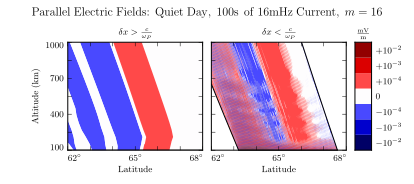
\includegraphics[width=\textwidth]{figures/inertial_length.pdf}
    \caption[Parallel Electric Fields by Perpendicular Grid Resolution]{
      The parallel electric field develops significant structure when the perpendicular grid resolution is smaller than the electron inertial length. Unfortunately, such runs are prohibitively expensive. The lower panel -- which still fails to resolve wave structure properly -- represents a 100-fold increase in computational time. 
    }
    \label{fig_inertial_length}
\end{figure}

Even so, the run presents a significant computational expense. Spread over 16 cores, a \SI{100}{\s} run on Tuna's usual grid takes well under an hour. The inertial-scale run barely finished in 96 hours, the cutoff at the Minnesota Supercomputing Institute\footnote{Runtime goes as the inverse square of grid resolution. Not only does finer resolution require more grid cells, but it also gives rise to proportionally smaller crossing times, imposing a smaller time step. }.

The snapshot shown in \cref{fig_inertial_length} uses a perpendicular grid resolution of \SI{0.7}{\km} at the Earthward edge, which just satisfies the Nyquist rate for the minimum inertial length of \SI{1.7}{\km}. It's still too coarse. There is clearly some small-scale structure developing in the ionosphere, but it's not well resolved. The large number of ``wigglies'' portends an imminent crash. 

Electron inertial effects present a promising first-principles-based approach to investigate parallel currents and electric fields associated with field line resonances. Unfortunately, because of the large differences in scale between Pc4 pulsations and the plasma oscillation, the proper deployment of inertial effects presents a prohibitive computational expense. For this reason, results presented in \cref{ch_results} make use of the core version of Tuna presented in \cref{sec_tuna}, which does not include the effects of electron inertia. 




%\endgroup

% %%%%%%%%%%%%%%%%%%%%%%%%%%%%%%%%%%%%%%%%%%%%%%%%%%%%%%%%%%%%%%%%%%%%%%%%%%%%%
% %%%%%%%%%%%%%%%%%%%%%%%%%%%%%%%%%%%%%%%%%%%%%%%%%%%%%%% Building on Mann 1995
% %%%%%%%%%%%%%%%%%%%%%%%%%%%%%%%%%%%%%%%%%%%%%%%%%%%%%%%%%%%%%%%%%%%%%%%%%%%%%

\chapter{Results}
  \label{ch_azm}

\todo{This chapter is the real moneymaker. The overarching motivation for this work is that Pc4 pulsations vary in interesting ways with respect to azimuthal modenumber, and that prior models have been unable to give a good picture of that behavior. }

%\todo{Do we every check E/B against $\Sigma_P / \mz$? }

%\todo{Do we see a difference between \vec{k} (momentum) and the group velocity? Poynting flux will always be pretty much along the field line, since $B_3$ is small and $E_3$ is zero, but the wave vector need not be. This is a question of coupling/converting to compressional waves, I guess. }

%\todo{Look at McKenzie and Westphal. Waves incident on the bow shock, etc, at weird angles. }

%\todo{Look at the E to B ratio. Compare to the \Alfven speed and to the height-integrated Pedersen conductivity. }

% =============================================================================
% =============================================================================
% =============================================================================
%\section{Electromagnetic Energy Gap}

%\todo{A preliminary search (and asking Bob) has not turned up anyone looking at this before, so it's hard to provide context. }

%Above, we considered the decay of energy from the poloidal mode to the toroidal mode. A natural follow up is, are there any other surprising trends in the distribution of energy?

%As it turns out, yes!

%In cases where the driving frequency does not line up with the local bounce frequency, energy doesn't accumulate particularly well in either the poloidal or the toroidal mode. Like a damped-driven oscillator, the system's behavior follows the input. 

%At low \azm, what energy there is divides itself more or less equally between the electric and magnetic fields. 

%As \azm increases, oddly, a gap appears. When the conductivity is high, the magnetic field holds more energy than the electric field. The disparity can be up to a factor of $\sim \num{3}$; that is, \SI{75}{\percent}. of the energy in the magnetic field, and \SI{25}{\percent} in the electric field. When conductivity is low, the opposite happens: energy concentrates in the electric field. 

%This lines up somewhat with what might be expected. When conductivity is low, it takes a larger electric field to induce the same current, and thus the same magnetic field. But it's not clear why this disparity only appears at large \azm, or why it does not appear when the driving is resonant. 

%Maybe it's a timing issue? A relationship between the bounce time (which is more or less indepedent of \azm) and the rotation time (which depends on \azm). 

%\todo{How is the compressional magnetic field brought into these calculations? It exists only at small \azm. It's never particularly large, it also gets added to the zeroth-order field before squaring. }

%\begin{figure}[H]
%    \centering
%    \includegraphics[width=\textwidth]{figures/U_BE_010mHz.pdf}
%    \caption[Current-Driven Electric and Magnetic Energy: 10mHz]{
%      In the absence of resonant driving, a disparity emerges at large \azm between the energy in the magnetic field and the energy in the electric field. The sign of the difference depends on the ionospheric conductivity. 
%    }
%    \label{fig_U_BE_010mHz}
%\end{figure}

%\begin{figure}[H]
%    \centering
%    \includegraphics[width=\textwidth]{figures/U_BE_022mHz.pdf}
%    \caption[Current-Driven Electric and Magnetic Energy: 22mHz]{
%      When driving is resonant, energy is distributed almost exactly half-and-half between the electric and magnetic fields, regardless of \azm. The rightmost profile still shows a gap, likely because the ionospheric conductivity in that model is low enough that nothing ever resonates. 
%    }
%    \label{fig_U_BE_022mHz}
%\end{figure}













  
% =============================================================================
% =============================================================================
% =============================================================================
\section{Finite Poloidal Lifetimes}
  \label{sec_lifetimes}

Radoski\cite{radoski_1974} looked at \Alfven waves, using a cylindrical coordinate system to imitate an ``unwrapped'' dipole. He argued that poloidal waves should asymptotically rotate to the toroidal mode. 

Mann\cite{mann_1995} performed some wave-in-a-box simulations and found the rotation time to be linear in modenumber: $\tau = \frac{d \lambda}{d \omega_A'}$, where $\lambda = \frac{\azm}{2 \pi r}$ and $\omega_A'$ is the spatial derivative of the \Alfven bounce frequency. Soon afterwards\cite{mann_1997}, he supported his simulations analytically. 

\todo{Crunch out $\frac{d \lambda}{d \omega_A'}$. Preliminary indications are that it doesn't translate well to a realistic grid, but let's double check. }

Ding\cite{ding_1995} ran simulations more-or-less concurrent with Mann's. Ding saw a rotation from poloidal to toroidal... then back again. It seems that the reversal was a spatial resolution issue. 

The aforementioned models made significant simplifying assumptions in terms of geometry and boundary conditions. 

Mann used straight field lines, a uniform \Alfven speed gradient, and perfectly conducting boundaries. 

Ding's simulation is nominally carried out in a dipole geometry, but the ionospheric boundary is at \SI{2.5}{\RE}. Boundaries are also perfectly conducting. 

That is, the results below offer a significantly higher level of realism than any past simulation (in part, of course, because computers are a lot better than they were 20 years ago). 

A dedicated 3D treatment of this problem is unlikely at present. Large azimuthal modenumbers are expensive to compute. That's the whole point! 

The energy is obtained by integrating (using the Jacobian to handle the grid properly) $U = \int dU = \int u \, dV$. Values are the log (base 10) of that, in the slightly odd units of gigajoules per radian. A factor of $2\pi$ wouldn't change anything, of course, but it seems inappropriate to integrate all the way around the sphere when Pc4s are longitudinally localized (a fact which was an important part of justifying a 2.5D approach). 

% -----------------------------------------------------------------------------
% -----------------------------------------------------------------------------
% -----------------------------------------------------------------------------
\subsection{High Conductivity}

In \cref{fig_U_day}, the rotation of energy from the poloidal mode to the toroidal mode is clear. Driving is strictly poloidal, yet the toroidal mode accumulates energy over time, and doesn't appear to give it back. The rotation happens faster for low-\azm simulations, qualitatively consistent with Mann's result; the time at which poloidal and toroidal energies are equal seems to even be linear in \azm, in line with his result. 

At least, this is the case on the dayside, where the ionosphere is highly conductive. 

\begin{figure}[H]
    \centering
    \includegraphics[width=\textwidth]{figures/U_1.pdf}
    \caption[Poloidal and Toroidal Energy: Active Day]{
      Driving -- delivered to the poloidal mode -- asymptotically rotates to the toroidal mode. The rate of rotation is strongly affected by the azimuthal modenumber. 
    }
    \label{fig_U_day}
\end{figure}

\todo{Talk about why this is exciting. }

\todo{Note that Mann looked specifically at second-harmonic waves. }

\todo{This result shows agreement with -- and significant refinement of -- Mann's findings. In the case of large-but-finite ionospheric conductivity, dipole geometry, and realistic \Alfven speed profile, energy does asymptotically rotate from the poloidal mode to the toroidal mode. The rotation rate is strongly affected by azimuthal modenumber and, in the case of large-but-finite \azm, has a characteristic timescale in the tens of periods. The present work furthermore demonstrates that the rotation rate is affected by driving frequency (did Mann talk about this at all, or just work in normalized time?) }

% -----------------------------------------------------------------------------
% -----------------------------------------------------------------------------
% -----------------------------------------------------------------------------
\subsection{Low Conductivity}

The picture on the nightside (where the ionospheric conductivity is low) is significantly different from the dayside (where it's high). 

Dissipation seems to outstrip rotation. Energy does not accumulate over numerous driving periods, as would be expected in resonance; it follows the driving up and down, as a damped-driven oscillator. 

There is evidence that the rotation is still trying to happen. At low \azm, energy is distributed between the poloidal and toroidal mode before dissipating; at high \azm, the energy dissipates straight out of the poloidal mode, never having had a chance to rotate. 

\begin{figure}[H]
    \centering
    \includegraphics[width=\textwidth]{figures/U_4.pdf}
    \caption[Poloidal and Toroidal Energy: Quiet Night]{
      Driving is applied to the poloidal electric field. There is some rotation of energy to the toroidal mode (and less at high azimuthal modenumber), but the low ionospheric conductivity prevents energy from accumulating over time. 
    }
    \label{fig_U_night}
\end{figure}

\todo{Why is this exciting? }

\todo{Previous considerations of poloidal lifetimes have been limited to the high conductivity regime. The present work demonstrates that the low conductivity regime exhibits qualitative differences. Ionospheric conductivity on the nightside is low enough that resonance does not develop, even in the case of ongoing driving. The dissipation timescale is comparable to the rotation timescale. Rather than aymoptotically accumulating energy in the toroidal mode, the oscillator asymptotically oscillates following the driving. This is relevant to the question of day-night asymmetry in the observation of field line resonances. }


  
% =============================================================================
% =============================================================================
% =============================================================================
\section{Spatial Distribution of Energy}
  \label{sec_shells}

Looking a bit deeper, it's possible to comment on the structure of the poloidal and toroidal modes, not just their magnitudes. The following commentary addresses the dayside; on the nightside, there's never much by the way of resonance. 

In \cref{fig_resonant_driving,fig_nonresonant_driving}, electromagnetic energy is binned by field line, averaged over volume (again, with respect to the Jacobian), and plotted as contours. All plots share a color scale. 

The poloidal mode and the toroidal mode exhibit qualitatively different behavior, related to the fact that energy rotates from poloidal to toroidal, and not back. 

At low \azm, energy rotates out of the poloidal mode so quickly that no resonance can form. 

At high \azm, the \Alfven wave is guided. If the driving frequency lines up with the resonant frequency where it's delivered, the poloidal mode resonates strongly. Otherwise, again, no energy accumulates. 

In no case does the poloidal mode demonstrate the ability to move energy across magnetic field lines. 

On the other hand, the toroidal mode does resonate, even if the driving isn't resonant (though in that case the response is of course stronger). The toroidal mode transports energy across field lines until it encounters resonance, then accumulates energy there. Often, resonances are seen in multiple locations due to the non-monotonic \Alfven bounce frequency (recall \cref{fig_fa}) as a function of $L$. 

% -----------------------------------------------------------------------------
% -----------------------------------------------------------------------------
% -----------------------------------------------------------------------------
\subsection{Resonant Driving}

\begin{figure}[H]
    \centering
    \includegraphics[width=\textwidth]{figures/layers_22mHz_1.pdf}
    \caption[Poloidal and Toroidal Energy Distribution: Resonant Driving]{
      If \azm is small, energy rotates to the toroidal mode too fast to form a poloidal resonance. If \azm is large, the \Alfven wave is guided, so it resonates only if the driving frequency lines up with the resonant frequency where it's applied. The result is just one big -- or perhaps even giant -- pulsation. If the driving lines up with a nearby field line, the toroidal mode goes crazy! Resonance inside the plasmasphere. Resonance at the plasmapause. Resonance at the driving location. And (weak) attempt at a higher harmonic further out. 
    }
    \label{fig_resonant_driving}
\end{figure}

\todo{Why is this exciting? }

\todo{Driving from inside the magnetosphere is novel. }

% -----------------------------------------------------------------------------
% -----------------------------------------------------------------------------
% -----------------------------------------------------------------------------
\subsection{Nonresonant Driving}

\begin{figure}[H]
    \centering
    \includegraphics[width=\textwidth]{figures/layers_13mHz_2.pdf}
    \caption[Poloidal and Toroidal Energy Distribution: Nonresonant Driving]{
      When the driving frequency doesn't line up with the location where it's delivered, there's basically no response. There is no movement of energy to a resonant field line, so no energy can accumulate over the course of multiple rounds of driving. Even when not driven resonantly, the toroidal mode still makes the best of its situation. It steals what energy it can from the poloidal mode, carries it to the resonant $L$-shell, and gets to work. (In contrast, recall from \cref{fig_resonant_driving}, in this situation the poloidal mode just does not accumulate energy.)
    }
    \label{fig_nonresonant_driving}
\end{figure}

\todo{Why is this exciting? }


  
% =============================================================================
% =============================================================================
% =============================================================================
\section{Significance for Giant Pulsations}
  \label{sec_pgs}

Giant pulsations are (probably\cite{takahashi_2011}) fundamental mode poloidal Pc4 pulsations with frequencies around \SI{10}{\mHz} and azimuthal modenumbers around \num{20}. They are large, and can sometimes be observed on the ground. 

While this model makes no particular distinction between a giant pulsation and any other Pc4, the above results do line up with giant pulsation observations. 

Giant pulsations aren't seen at small \azm. As shown in \cref{sec_lifetimes}, low-\azm poloidal modes rotate to the toroidal mode too quickly to resonate effectively, even in the case of continuous driving at a locally-resonant frequency. The sweet spot seems to be around $\azm = 20$, more or less the same point where resonance becomes visible in \cref{fig_resonant_driving}. Admittedly, giant pulsations are typically closer to \SI{10}{\mHz} than \SI{22}{\mHz}. It seems likely that qualitatively similar results would be encountered if the driving were moved to an $L$-shell with a bounce time of \SI{10}{\mHz}. 

% -----------------------------------------------------------------------------
% -----------------------------------------------------------------------------
% -----------------------------------------------------------------------------
\subsection{Ground Signatures}

\todo{\cite{takahashi_2011} talks significantly about the east-west polarization. }

Giant pulsations are seen at very large \azm, though not on the ground\cite{takahashi_2013}, due to damping by the ionosphere. 

Giant pulsations are most common on the dayside (particularly the morningside), during geomagnetically quiet times. Giant pulsation ground signatures are noted for their predisposition towards east-west polarization. 

In \cref{fig_ground_signatures}, the strongest east-west ground signatures is obtained on the geomagnetically quiet dayside, at \azm of 16 and 32. 

This seems to be a giant pulsation ``sweet spot'': the poloidal mode becomes stronger as \azm increases, but the ionospheric damping also increases. 

\begin{figure}[H]
    \centering
    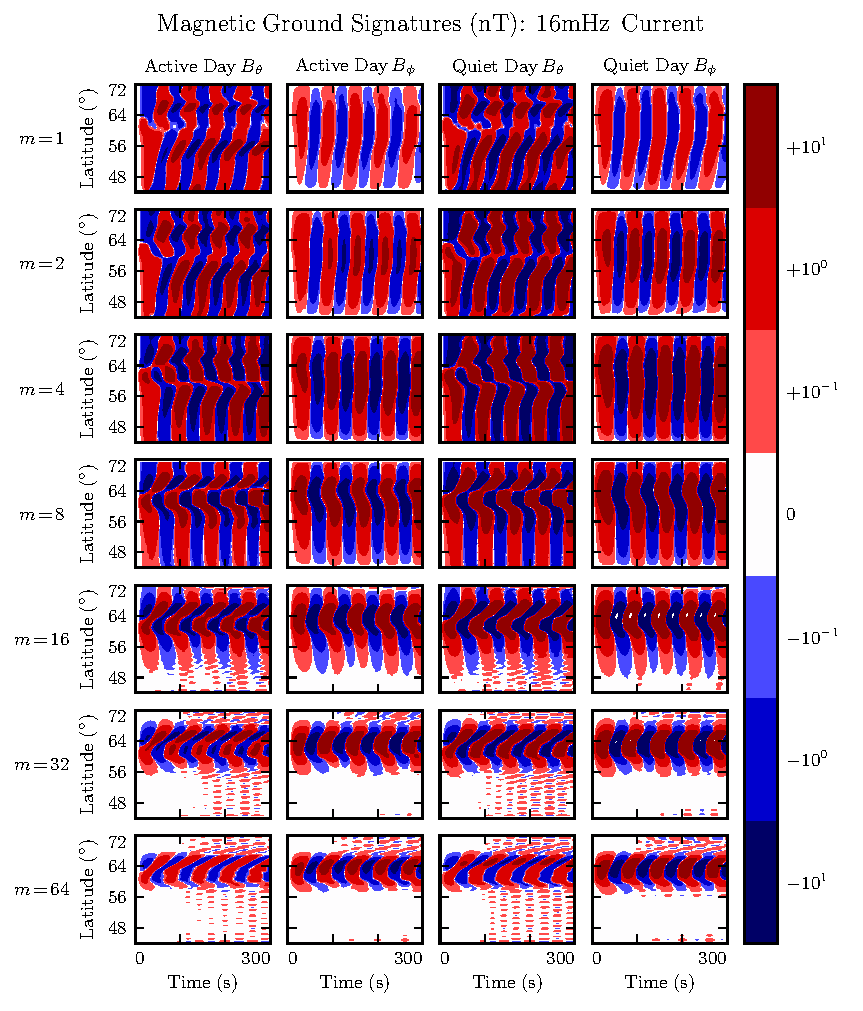
\includegraphics[width=\textwidth]{figures/ground_16mHz.pdf}
    \caption[Dayside Ground Magnetic Fields]{
      The east-west component of magnetic ground signatures is peaked on the geomagnetically quiet dayside, at modenumbers around 16 to 32. This coincides nicely with observations of giant pulsations. Like the east-west component, the north-south ground signature is strongest on the quiet dayside; however, unlike the east-west component, the north-south component is weak when the modenumber is large. 
    }
    \label{fig_ground_signatures}
\end{figure}

Giant pulsations are monochromatic, and can be accompanied by ``multiharmonic toroidal waves''\cite{takahashi_2011}. Per \cref{sec_shells}, this is about what would be expected from a mishmash of poloidal driving. Poloidal modes of all frequencies rotate into the toroidal mode; resonant poloidal modes resonate; non-resonant poloidal modes become evanescent. 

Giant pulsations often drift azimuthally. This model can't resolve azimuthal drift directly, of course, but can fake it by looking at complex phase. There has been some indication (not shown) of complex phase rotation in ground magnetic fields. However, at the boundary, it's difficult to disentangle which values are imaginary to indicate an azimuthal offset, and which are imaginary because of Hall coupling. Investigation is ongoing. 




% %%%%%%%%%%%%%%%%%%%%%%%%%%%%%%%%%%%%%%%%%%%%%%%%%%%%%%%%%%%%%%%%%%%%%%%%%%%%%
% %%%%%%%%%%%%%%%%%%%%%%%%%%%%%%%%%%%%%%%%%%%%% Validate the Model Against RBSP
% %%%%%%%%%%%%%%%%%%%%%%%%%%%%%%%%%%%%%%%%%%%%%%%%%%%%%%%%%%%%%%%%%%%%%%%%%%%%%

\chapter{Observations}
  \label{ch_rbsp}

\todo{Talk about recent surveys by Dai\cite{dai_2015} and Motoba\cite{motoba_2015}. Note that they skirt the issue of the fundamental mode in general. Everyone talks about how Pgs are rare... but how rare are they compared to the fundamenal poloidal Pc4 in general? }







  
% =============================================================================
% =============================================================================
% =============================================================================
\section{Event Selection}

% -----------------------------------------------------------------------------
% -----------------------------------------------------------------------------
% -----------------------------------------------------------------------------
\subsection{Identifying the Fundamental Harmonic}

Takahashi\cite{takahashi_2013} spells this out explicitly. Fundamental mode, south of the equator, V should lead B by 90 degrees. 

Per Takahashi\cite{takahashi_2011}, phase lag can be used to distinguish the fundamental harmonic from the second harmonic. 

Chisham and Orr\cite{chisham_1991} argue that around \SI{7}{\RE}, frequency around \SI{10}{\mHz} precludes higher harmonics. Or maybe look at \cite{green_1985}?

Green\cite{green_1979} and Cummings\cite{cummings_1969} talk about the frequencies for ideal toroidal modes. 

Dai\cite{dai_2015} says to look at \cite{takahashi_2011} and \cite{dai_2013} for unambiguous identification of the fundamental mode. 


  
% =============================================================================
% =============================================================================
% =============================================================================
\section{Something Something Results}

% -----------------------------------------------------------------------------
% -----------------------------------------------------------------------------
% -----------------------------------------------------------------------------
\subsection{Something Something Results}





% %%%%%%%%%%%%%%%%%%%%%%%%%%%%%%%%%%%%%%%%%%%%%%%%%%%%%%%%%%%%%%%%%%%%%%%%%%%%%
% %%%%%%%%%%%%%%%%%%%%%%%%%%%%%%%%%%%%%%%%%%%%%%%%%%%%%%%%%%%%%%%%%% Conclusion
% %%%%%%%%%%%%%%%%%%%%%%%%%%%%%%%%%%%%%%%%%%%%%%%%%%%%%%%%%%%%%%%%%%%%%%%%%%%%%

\chapter{Conclusion}
  \label{ch_conclusion}



  % =============================================================================
% =============================================================================
% =============================================================================
\section{Summary of Results}

\todo{Write this. }


  \include{chapters/sec_future}

% Bibliography
\bibliography{dissertation}

% Appendices
\appendix

% %%%%%%%%%%%%%%%%%%%%%%%%%%%%%%%%%%%%%%%%%%%%%%%%%%%%%%%%%%%%%%%%%%%%%%%%%%%%%
% %%%%%%%%%%%%%%%%%%%%%%%%%%%%%%%%%%%%%%%%%%%%% Appendix: Differential Geometry
% %%%%%%%%%%%%%%%%%%%%%%%%%%%%%%%%%%%%%%%%%%%%%%%%%%%%%%%%%%%%%%%%%%%%%%%%%%%%%

\chapter{Differential Geometry}
\label{app_geometry}

\todo{Not sure that a glossary or list of acronyms will be necessary, but here are the examples from the template. }

\section{Glossary}
\label{jargonapp}
\begin{itemize}
\item \textbf{Cosmic-Ray Muon} (\textbf{CR $\mu$}) -- A muon coming from
the abundant energetic particles originating outside of the Earth's
atmosphere.
\end{itemize}

\section{Acronyms}
\label{acronymsec}

% Heading for the first page
\begin{longtable}{p{0.25\textwidth} p{0.75\textwidth}}
\caption{Acronyms} \label{tab:acronyms} \\

\toprule
Acronym & Meaning \\
\midrule
\endfirsthead

% Heading for all subsequent pages
\multicolumn{2}{l}{\textit{\tablename\ \thetable{} -- Continued from previous page}} \\
\toprule
Acronym & Meaning \\
\midrule
\endhead

% Footer for each page that wraps over to the next
\multicolumn{2}{r}{\textit{Continued on next page}} \\
\bottomrule
\endfoot

% Footer for the end of the table
\bottomrule
\endlastfoot

% End table formatting

CR$\mu$ & Cosmic-Ray Muon \\

\end{longtable}



%% %%%%%%%%%%%%%%%%%%%%%%%%%%%%%%%%%%%%%%%%%%%%%%%%%%%%%%%%%%%%%%%%%%%%%%%%%%%%%
% %%%%%%%%%%%%%%%%%%%%%%%%%%%%%%%%%%%%%%%%%%%%%%% Appendix: Integrating Factors
% %%%%%%%%%%%%%%%%%%%%%%%%%%%%%%%%%%%%%%%%%%%%%%%%%%%%%%%%%%%%%%%%%%%%%%%%%%%%%








\chapter{Integrating Factors}
\label{app_integrating}

Start with differential equation of the form:

\begin{align}
  \frac{\partial}{\partial t} X(t) + \alpha X(t) &= \beta
\end{align}

Multiply by the integrating factor, then group terms: 

\begin{align}
  \exp (\alpha \; t) \frac{\partial}{\partial t} X(t) + \alpha \exp(\alpha \; t) X(t) &= \beta \exp(\alpha \; t) \\
  \frac{\partial}{\partial t} \big[ \exp(\alpha t) X(t) \big] &= \beta \exp(\alpha t)
\end{align}

Integrate from 0 to $\delta t$, assuming that $\beta$ is constant in time or varies slowly. 

\begin{align}
  \int^{\delta t}_0 dt \frac{\partial}{\partial t} \big[ \exp(\alpha t) X(t) \big] &= \int^{\delta t}_0 dt \beta \exp(\alpha t) \\
  \exp (\alpha \deltat) X(\deltat) - X(0) &= \deltat \beta ( \frac{\deltat}{2} ) \exp ( \alpha \frac{\deltat}{2} )
\end{align}

Then rearrange to solve for the new value of X:

\begin{align}
  X(\delta t) &= X(0) \exp ( -\alpha \delta t ) + \delta t \beta ( \frac{\delta t}{2} ) \exp ( -\alpha \frac{\delta t}{2} )
\end{align}

Done. 


% End the Document
\end{document}




